% =====================================================================
%  main.tex -- 主文档
%  编译: xelatex main.tex  (需两次以上以生成目录与交叉引用)
% =====================================================================
\documentclass[UTF8,a4paper,11pt]{ctexart}
% =====================================================================
%  style.tex -- 公共宏包、版式与代码排版设置
% =====================================================================
\usepackage[a4paper,left=2.0cm,right=2.0cm,top=2.4cm,bottom=2.2cm,headsep=0.6cm]{geometry}
\usepackage{xcolor}
\usepackage{listings}
\usepackage{booktabs}
\usepackage{longtable}
\usepackage{array}
\usepackage{amsmath,amssymb}
\usepackage{caption}
\usepackage{enumitem}
\usepackage{fancyhdr}
\usepackage{tikz}
\usetikzlibrary{positioning,arrows.meta,shapes.geometric,fit,backgrounds}
\usepackage[colorlinks=true,linkcolor=blue!55!black,urlcolor=blue!55!black,citecolor=blue!55!black,
            bookmarksnumbered=true]{hyperref}

% ---------- 颜色 ----------
\definecolor{codebg}{gray}{0.985}
\definecolor{codeframe}{gray}{0.62}
\definecolor{kw}{RGB}{0,80,160}
\definecolor{cmt}{RGB}{0,110,90}
\definecolor{str}{RGB}{150,60,0}
\definecolor{warnbg}{RGB}{255,244,224}
\definecolor{warnframe}{RGB}{200,120,0}
\definecolor{tipbg}{RGB}{232,244,255}
\definecolor{tipframe}{RGB}{30,90,170}

% ---------- 代码块样式 ----------
\lstdefinestyle{vcode}{
  language=Verilog,
  basicstyle=\ttfamily\scriptsize,
  keywordstyle=\color{kw}\bfseries,
  commentstyle=\color{cmt},
  stringstyle=\color{str},
  numbers=left, numberstyle=\tiny\color{gray}, numbersep=6pt,
  backgroundcolor=\color{codebg}, frame=single, rulecolor=\color{codeframe},
  framexleftmargin=1.2em, xleftmargin=1.6em,
  columns=fullflexible, keepspaces=true, showstringspaces=false,
  tabsize=4, breaklines=true, breakatwhitespace=false,
  extendedchars=true, inputencoding=utf8,
  aboveskip=1.0em, belowskip=0.6em,
  upquote=true
}
\lstdefinestyle{vsnip}{
  language=Verilog,
  basicstyle=\ttfamily\small,
  keywordstyle=\color{kw}\bfseries,
  commentstyle=\color{cmt},
  stringstyle=\color{str},
  numbers=none,
  backgroundcolor=\color{codebg}, frame=single, rulecolor=\color{codeframe},
  framexleftmargin=0.6em, xleftmargin=1.0em,
  columns=fullflexible, keepspaces=true, showstringspaces=false,
  tabsize=4, breaklines=true, breakatwhitespace=false,
  extendedchars=true, inputencoding=utf8,
  aboveskip=0.8em, belowskip=0.5em
}
\lstdefinestyle{cfgcode}{
  basicstyle=\ttfamily\scriptsize,
  numbers=left, numberstyle=\tiny\color{gray},
  backgroundcolor=\color{codebg}, frame=single, rulecolor=\color{codeframe},
  framexleftmargin=1.2em, xleftmargin=1.6em,
  columns=fullflexible, keepspaces=true, showstringspaces=false,
  breaklines=true, extendedchars=true, inputencoding=utf8
}

% ---------- 标识符排版 ----------
\DeclareRobustCommand{\sig}[1]{\texttt{\detokenize{#1}}}
\DeclareRobustCommand{\file}[1]{\texttt{\detokenize{#1}}}
\DeclareRobustCommand{\reg}[1]{\sig{#1}}

% ---------- 提示框(环境形式, 内部可用段落/公式/列表) ----------
\newsavebox{\noteboxsave}
\newenvironment{warnbox}
  {\par\medskip\noindent\begin{lrbox}{\noteboxsave}%
   \begin{minipage}{\dimexpr\linewidth-2\fboxsep-2\fboxrule}\small}
  {\end{minipage}\end{lrbox}%
   \fcolorbox{warnframe}{warnbg}{\usebox{\noteboxsave}}\par\smallskip}
\newenvironment{tipbox}
  {\par\medskip\noindent\begin{lrbox}{\noteboxsave}%
   \begin{minipage}{\dimexpr\linewidth-2\fboxsep-2\fboxrule}\small}
  {\end{minipage}\end{lrbox}%
   \fcolorbox{tipframe}{tipbg}{\usebox{\noteboxsave}}\par\smallskip}

% ---------- 表格辅助 ----------
\newcolumntype{L}[1]{>{\raggedright\arraybackslash}p{#1}}
\newcolumntype{C}[1]{>{\centering\arraybackslash}p{#1}}
\newcommand{\tabfont}{\small}
\captionsetup{font=small,labelfont=bf}
\setlength{\parskip}{0.25em}
\renewcommand{\arraystretch}{1.15}

% ---------- 页眉页脚 ----------
\pagestyle{fancy}
\fancyhf{}
\fancyhead[L]{\small 高云 GW5A-25A 的 \texttt{project\_2025\_11\_07} 工程代码逐层解析}
\fancyhead[R]{\small \thepage}
\renewcommand{\headrulewidth}{0.3pt}

% ---------- 目录深度 ----------
\setcounter{tocdepth}{3}
\setcounter{secnumdepth}{3}

% ---------- 常用宏 ----------
\newcommand{\cntmax}[1]{\sig{#1}}
\newcommand{\unit}[1]{\,\mathrm{#1}}


\title{\bfseries 高云 GW5A-25A FPGA 工程\\[2mm]
       \texttt{project\_2025\_11\_07} 代码逐层解析与注释说明}
\author{FPGA 代码解读报告}
\date{2026 年 10 月}

\begin{document}

% ------------------------- 封面 -------------------------
\begin{titlepage}
\centering
\vspace*{2.2cm}
{\Huge\bfseries 高云 GW5A-25A FPGA 工程}\\[4mm]
{\Huge\bfseries \texttt{project\_2025\_11\_07}}\\[6mm]
{\LARGE 代码逐层解析与注释说明}\\[18mm]
\begin{tabular}{rl}
\toprule
器件型号 & \sig{GW5A-LV25UG324C2/I1}（\sig{GW5A-25A}，UBGA324，速度等级 2）\\
目标板卡 & AD/DA 采集 + 串口 + 数码管 + ADRC 控制演示板\\
顶层模块 & \texttt{adda\_scope\_top}（\file{src/vga/adda_scope_top.v}，含 VGA 示波器）\\
工程文件 & \file{project_2025_11_07.gprj}（Gowin EDA V1.9.9 64-bit）\\
对照工程 & \file{FPGA_TD/project_2025_11_07_TD.al}（Anlogic TD 6.0.3 浏览用容器）\\
修复分支 & \file{fix/review-p1-p11}（第 17 章，main 保持原样）\\
代码仓库 & \url{https://github.com/starfruitsz/FPGA}\\
文档版本 & v1.1（新增第 15--17 章）\\
生成日期 & 2026-10-29 \\
\bottomrule
\end{tabular}

\vfill
{\small 本报告覆盖工程中\textbf{全部} Verilog 源文件、IP 文件与物理约束文件；\\
每个文件按“模块接口 $\rightarrow$ 语句块 $\rightarrow$ 关键语句/信号”三级层次逐块解析，\\
并给出数值、时序与设计意图说明。所有源码均已在原位置添加中文注释，\\
注释前后代码的 Verilog 词法内容经脚本比对完全一致（仅新增注释）。}
\end{titlepage}

\tableofcontents
\clearpage

% =====================================================================
%  ch01_overview.tex -- 第 1 章 工程总览
% =====================================================================
\section{工程总览}

\subsection{本报告的范围与方法}

本报告针对 \file{project_2025_11_07} 这一 Gowin（高云）FPGA 工程，逐文件、逐语句块地
解析其 RTL 设计。分析对象为工程文件中列出的全部 11 个 Verilog 源文件、2 个 IP 生成文件、
1 个物理约束文件，以及工程目录中附带的 2 个 IP 例化模板：

\begin{center}
\small
\begin{tabular}{llc}
\toprule
类别 & 文件 & 是否进入网表\\
\midrule
顶层 & \file{src/adda.v} & 是（Top）\\
算法 & \file{src/rtl.v}、\file{src/eso.v} & 是\\
外设 & \file{src/uart_rx.v}、\file{src/uart_tx.v} & 是\\
显示 & \file{src/seg.v}、\file{src/bcd.v} & 是\\
基础 & \file{src/key.v}、\file{src/divider.v} & 是\\
IP & \file{src/gowin_pll/gowin_pll.v} & 否（未例化）\\
IP & \file{src/fifo_top/fifo_top.v} & 否（未例化）\\
约束 & \file{src/project_2025_11_07.cst} & 引脚/电平\\
模板 & \file{src/gowin_pll/gowin_pll_tmp.v}、\file{src/fifo_top/fifo_top_tmp.v} & 否（仅供查阅）\\
\bottomrule
\end{tabular}
\end{center}

“进入网表”一列并非主观判断，而是由三处证据共同确认：综合资源报告
\file{syn_rsc.xml} 中只出现 7 个子模块；PnR 报告 \file{rpt.txt} 中 PLL 占用为
\sig{0/6}、BSRAM 占用为 0\%；以及 \file{adda.v} 中 \sig{Gowin_PLL}、\sig{fifo_top}
的例化代码被注释符包裹（完整路径见第 1.2 节的目录说明）。

解析方法遵循“自顶向下、逐块下钻”的原则，每一章的结构固定为：
\begin{enumerate}[leftmargin=2em,itemsep=2pt]
  \item \textbf{文件信息}：路径、模块名、实例名、行数、时序模板；
  \item \textbf{模块接口（第 1 层）}：端口表、参数表；
  \item \textbf{内部结构（第 2 层）}：寄存器/连线清单与语句块索引；
  \item \textbf{语句块解析（第 3 层）}：每块给出现行代码、逐信号解释、数值与时序推演；
  \item \textbf{要点与风险}：设计意图、隐含假设、潜在缺陷。
\end{enumerate}

\subsection{工程来源、工具链与“用 TD 打开”的说明}

\subsubsection{原始工程}

工程由 Gowin EDA（云源软件）V1.9.9 64-bit 生成，工程主文件为
\file{project_2025_11_07.gprj}，其 \sig{<Device>} 节点写明了器件：

\begin{lstlisting}[style=cfgcode,numbers=none]
<Device name="GW5A-25A" pn="GW5A-LV25UG324C2/I1">gw5a25a-008</Device>
\end{lstlisting}

综合工程文件还给出了封装与速度等级：
\begin{lstlisting}[style=cfgcode,numbers=none]
<Device id="GW5A-25A" package="UBGA324" speed="2" partNumber="GW5A-LV25UG324C2/I1"/>
\end{lstlisting}

\subsubsection{关于用安路 TD 打开该工程}

这里需要明确一个前提：\textbf{安路 TangDynasty（TD）无法直接打开高云的 \texttt{.gprj} 工程}。
两者是不同厂商的私有工程格式（高云 \sig{.gprj} / 安路 \sig{.al}），器件库、原语、IP 格式、
约束语言（高云 \sig{.cst} 与安路 \sig{.adc}/\sig{.fdc}）均不兼容。经检查，本机安装的是
\textbf{TD 6.0.3 PHX SP2}，其器件数据库 \file{D:\textbackslash FPGA\textbackslash arch\textbackslash device_resource\textbackslash device_resource.csv}
只包含 \sig{ph1}（13 个）与 \sig{ph2}（2 个）两个 Phoenix 系列，不含 GW5A 或任何高云器件。

因此本次采用“\textbf{同名工程容器}”的方案：用 TD 的 Tcl 接口
（\file{td_commands_prompt.exe -nogui}）新建了一个与源码同名的 TD 工程
\file{FPGA_TD/project_2025_11_07_TD.al}，器件选用 TD 6.0.3 中规模最小、封装同为 324 球的
\sig{PH1A60GEG324-3}，再把 11 个 Verilog 源文件以\textbf{引用方式}（不复制）加入工程。
这样 TD 的层次树、源码浏览器、交叉引用功能都能用于阅读和注释本工程的代码，而
\textbf{原始高云工程完全未被改动}。

\begin{figure}[htbp]
\centering
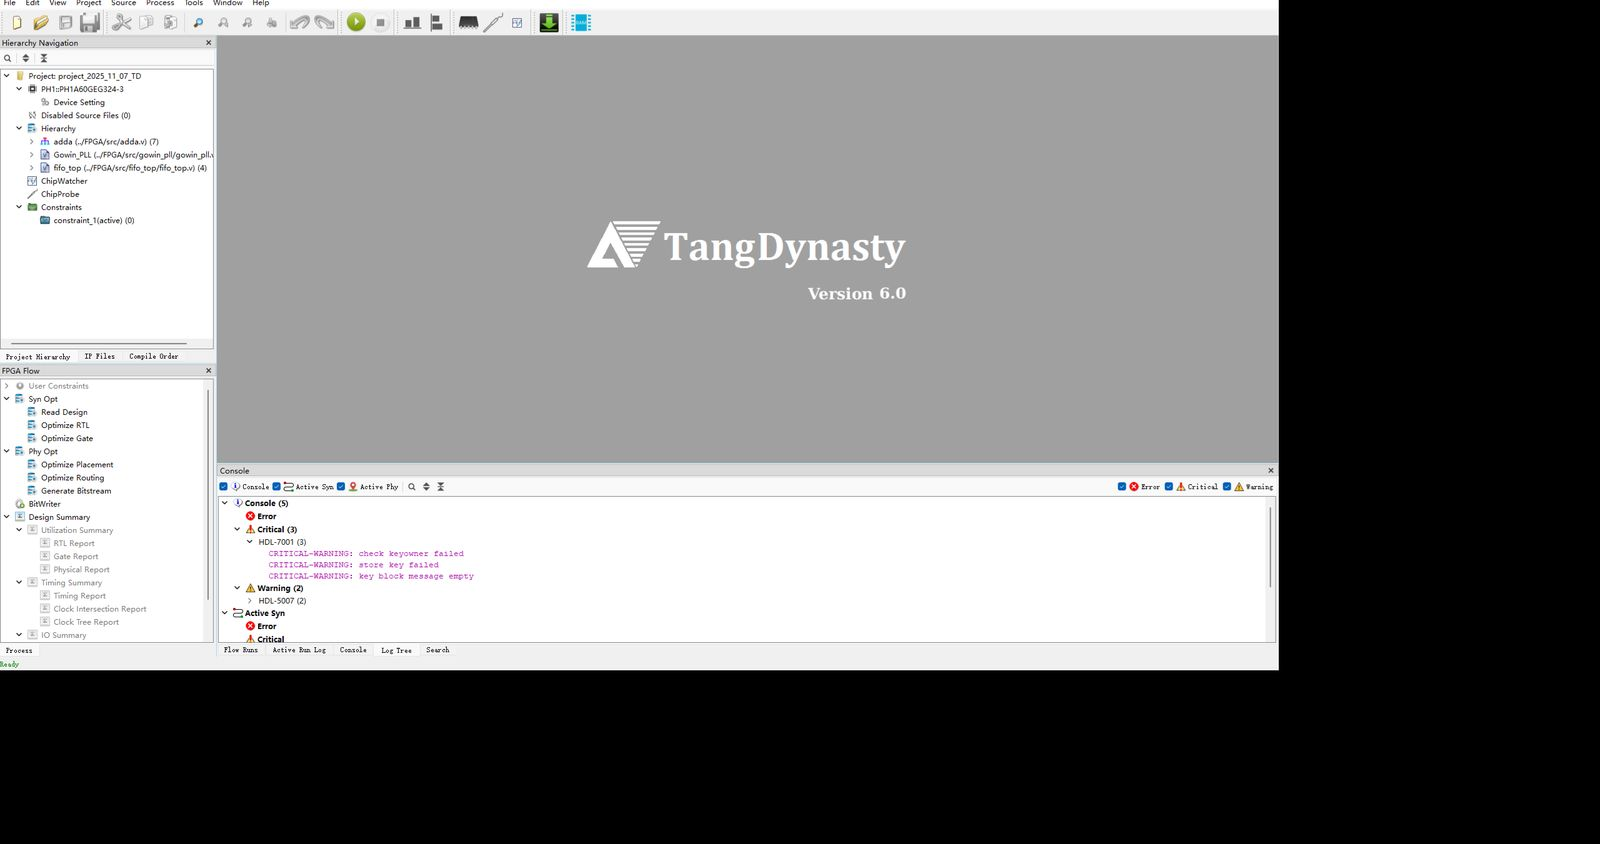
\includegraphics[width=0.92\linewidth]{figs/TD_open_project.jpg}
\caption{TD 6.0.3 打开同名工程容器后的界面：左侧 Hierarchy Navigation 已经识别出
\sig{adda (7)}、\sig{Gowin_PLL (1)}、\sig{fifo_top (4)} 三个层次根，说明全部源文件均被正确解析。}
\label{fig:td-open}
\end{figure}

\begin{tipbox}
\textbf{为什么层次树里 \sig{adda} 只有 7 个子节点？}
因为顶层只例化了 7 个模块（key、seg、rtl、eso、uart\_rx、uart\_tx、divider）。
\sig{Gowin_PLL} 与 \sig{fifo_top} 虽然被 TD 解析并单独列在层次树中，但它们是“未被例化的
孤立模块”，不会出现在 \sig{adda} 之下，也不会进入综合网表——这与高云综合报告的结论一致。
\end{tipbox}

\begin{warnbox}
\textbf{注意}：TD 容器工程只用于“阅读/结构化浏览”代码，\textbf{不要}用它做综合或生成码流。
一方面它选用的是安路 PH1 器件，与板上的 GW5A-25A 引脚、电气属性完全不同；另一方面
\sig{gowin_pll.v} 里的 \sig{PLLA} 原语和 \sig{fifo_top.v} 里加密的 FIFO 都不属于安路器件库。
若需要重新编译，应回到 Gowin EDA 打开原始 \sig{.gprj}。
\end{warnbox}

\subsection{器件与资源}

\begin{table}[htbp]
\centering
\small
\caption{GW5A-LV25UG324C2/I1 的容量与本工程占用}
\begin{tabular}{lrr}
\toprule
资源 & 器件容量 & 本工程占用\\
\midrule
LUT / ALU / ROM16（逻辑） & 23\,040 & 575（2\%）\\
寄存器（FF） & 23\,685 & 375（2\%）\\
CLS（逻辑簇） & 11\,520 & 405（4\%）\\
DSP（MULTALU27X18） & 28 & 7（25\%）\\
PLL & 6 & 0（0\%）\\
BSRAM & 若干 & 0（0\%）\\
I/O 端口 & — & 44（其中 42 个实际布出 Buffer）\\
\bottomrule
\end{tabular}
\end{table}

该器件属于 Arora V（GW5A）系列 22nm 工艺的入门型号，324 球 UBGA 封装，速度等级 2，
工业级/商业级双标注（C2/I1）。工程中真正消耗资源的核心是 \sig{eso.v} 的 9 个乘法器
（映射为 7 个 MULTALU27X18）与 \sig{rtl.v} 的两个除法器，其余模块都是控制/IO 逻辑。

\subsection{模块层次与文件对应关系}

\begin{figure}[htbp]
\centering
\begin{minipage}{0.9\linewidth}
\begin{verbatim}
adda  (src/adda.v)                              <- 顶层 / Top Module
 |-- key_inst      : key      (src/key.v)        按键消抖 20ms
 |-- seg_inst      : seg      (src/seg.v)        数码管动态扫描
 |    `-- bcd_8421 : bcd      (src/bcd.v)        二进制 -> 3 位 BCD
 |-- adc_inst      : rtl      (src/rtl.v)        中值滤波 + 电压换算
 |-- eso_inst      : eso      (src/eso.v)        扩展状态观测器 (ADRC)
 |-- uart_rx_inst  : uart_rx  (src/uart_rx.v)    串口接收 (8N1)
 |-- uart_tx_inst  : uart_tx  (src/uart_tx.v)    串口发送 (16bit)
 `-- divider_inst  : divider  (src/divider.v)    1kHz 分频

未例化(只在工程文件列表里): Gowin_PLL (gowin_pll.v) / fifo_top (fifo_top.v)
\end{verbatim}
\end{minipage}
\caption{模块层次树。带 \texttt{--} 前缀的是实例名，括号内为源文件。}
\label{fig:hier}
\end{figure}

\begin{table}[htbp]
\centering
\small
\caption{例化关系与实例名一览}
\begin{tabular}{llll}
\toprule
父模块 & 子模块 & 实例名 & 作用\\
\midrule
adda & key & key\_inst & 按键消抖 \\
adda & seg & seg\_inst & 数码管扫描显示 \\
seg & bcd & bcd\_8421 & 二进制转 BCD \\
adda & rtl & adc\_inst & 中值/电压换算 \\
adda & eso & eso\_inst & 扩展状态观测器 \\
adda & uart\_rx & uart\_rx\_inst & 串口接收 \\
adda & uart\_tx & uart\_tx\_inst & 串口发送 \\
adda & divider & divider\_inst & 1kHz 分频 \\
\bottomrule
\end{tabular}
\end{table}

\subsection{数据流与控制流}

系统是一套“AD 采样 $\rightarrow$ 数字化处理 $\rightarrow$ DA 回放 + 显示 + 串口上报 + 上位机在线调参”
的闭环演示平台：

\begin{figure}[htbp]
\centering
\begin{minipage}{0.95\linewidth}
\begin{verbatim}
  [外部 ADC] --ad_date[9:0]--> rtl (中值/电压) --sign--> seg(+bcd) --> 数码管
  [外部 ADC] --ad_date[9:0]--> date_y(=ad_date-512) --> eso(1kHz)
                --date_u--> (~u + 512) --> DAC ad_out[9:0]
  [上位机 rx] --Axxx/Bxxx--> uart_rx --> 16bit 组帧 --> c_date/k_date --> eso
  [按键 key_in] --> key --> key_out --> 选择 ad_out 的数据来源
  [ad_date] --> uart_tx --> tx (115200, 8N1, 每帧 182us)
  [sys_clk 50MHz] --> divider --> ad_clk1/da_clk1 (1kHz) --> eso 采样时钟
\end{verbatim}
\end{minipage}
\caption{数据流与控制关系（省略复位线与时钟树细节）。}
\label{fig:dataflow}
\end{figure}

\begin{table}[htbp]
\centering
\small
\caption{关键信号与跨模块连接}
\begin{tabular}{lp{3.2cm}p{6.4cm}}
\toprule
信号 & 位宽/类型 & 说明\\
\midrule
\sig{ad_date[9:0]} & 10bit 无符号 & 外部 ADC 并行码值（偏移二进制，中点 512）\\
\sig{date_y} & 10bit 有符号 & \sig{ad_date-512}，把中点移到零，送 ESO 的误差输入\\
\sig{date_u} & 10bit 有符号 & ESO 输出的控制量，同时回送 ESO 的 \sig{u_out} 形成反馈\\
\sig{ad_out[9:0]} & 10bit 无符号 & 送 DAC 的偏移二进制码，由按键选择“直通”或“控制量”\\
\sig{c_date/k_date} & 12bit & 串口下发的两个 ESO 参数（A 帧、B 帧的低 12 位）\\
\sig{po_data/po_flag} & 8bit/1bit & 串口接收字节与单周期有效脉冲\\
\sig{sign} & 1bit & 当前码值低于中值，数码管据此显示负号\\
\bottomrule
\end{tabular}
\end{table}

\subsection{时钟与复位策略}

\begin{table}[htbp]
\centering
\small
\caption{时钟域一览}
\begin{tabular}{llll}
\toprule
时钟 & 频率 & 来源 & 使用者\\
\midrule
\sig{sys_clk} & 50MHz & 板载有源晶振，引脚 T9 & adda、key、seg、uart\_rx、uart\_tx、divider\\
\sig{ad_clk1} & 1kHz & divider 由 \sig{sys_clk} 分频 & AD 芯片转换时钟、eso 运算时钟\\
\sig{da_clk1} & 1kHz & divider（与 \sig{ad_clk1} 同相） & DA 芯片转换时钟\\
\bottomrule
\end{tabular}
\end{table}

全设计只有一个异步复位 \sig{sys_rst_n}（低有效，引脚 A15），所有时序块都采用
“\sig{posedge clk or negedge rst_n}”的异步复位、同步释放风格（除 \sig{eso} 用
\sig{ad_clk} 作为时钟外）。由于 \sig{ad_clk1} 由 \sig{sys_clk} 分频而来，它与
\sig{sys_clk} 是同源的，1kHz 下不存在实际跨时钟域问题，但用“分频时钟”而非
“时钟使能”驱动的写法在更高频率下需要谨慎（见第 14 章）。

\subsection{参数与定点数约定汇总}

\begin{table}[htbp]
\centering
\small
\caption{全工程参数/常数}
\begin{tabular}{llll}
\toprule
位置 & 名称 & 取值 & 含义\\
\midrule
adda & \sig{CNT_DATA_MAX} & 1024 & 中值样本数（转发给 rtl 的约定值）\\
adda & \sig{CNT_MAX} & 1\,299\,999 & 26ms 定时器（仅驱动死信号 \sig{pi_flag}）\\
divider & \sig{cnt_max} & 24\,999 & $50\text{MHz}/(2\times25000)=1\text{kHz}$\\
key & \sig{CNT_MAX} & 999\,999 & 20ms 消抖时间\\
seg & \sig{CNT_MAX} & 23\,999 & 0.48ms 位扫描间隔\\
bcd & — & 22 拍 & 一次二进制转 BCD 的时钟数\\
uart\_rx/tx & \sig{UART_BPS} & 115\,200 & 波特率\\
uart\_rx/tx & \sig{CLK_FREQ} & 50\,000\,000 & 系统时钟，用于算分频\\
eso & \sig{B01/B02/B03} & 90 / 2700 / 27000 & 观测器增益（配合 $h=2^{-10}$）\\
eso & \sig{b0} & 5000 & 控制增益（配合 $>>13$）\\
eso & \sig{c} / \sig{k} & 150 / 20 & 状态误差反馈参数（可串口在线修改）\\
\bottomrule
\end{tabular}
\end{table}

工程中所有运算均为“整数 + 移位”的定点数，没有浮点。约定如下：
\begin{itemize}[leftmargin=2em,itemsep=1pt]
  \item \sig{rtl} 中电压量的标度为 $100\times$（即 1 LSB = 0.01V），满量程 $\pm2.0$V；
  \item \sig{eso} 中采样步长 $h=1/1024$ 由 \sig{>>>10} 实现，系数 \sig{B0x} 直接乘后右移；
  \item \sig{eso} 输出经 \sig{>>>15} 压缩后取低 10 位，映射到 DAC 的 0$\sim$1023 量程。
\end{itemize}

\subsection{代码风格与工程约定}

\begin{itemize}[leftmargin=2em,itemsep=2pt]
  \item \textbf{时序模板}：几乎所有状态块都是“复位分支 + else if 条件 + else 保持”结构，
        属于安全的默认保持型写法，综合后不会产生锁存器；
  \item \textbf{位宽}：大量使用 \sig{<= 1'b0} 给多位寄存器赋初值（例如
        \sig{data_reg<=1'b0}），Verilog 会自动零扩展，功能正确但不是严谨写法；
  \item \textbf{命名}：沿用“中文注释 + 拼音变量”（\sig{date}、\sig{pingj}、\sig{seg_date}），
        阅读时需要对照注释理解；
  \item \textbf{重复常量}：\sig{50_000_000} 在 uart 例化处出现两次，\sig{115200} 同样，
        若更换时钟需同步修改 PLL 参数、divider 参数与 uart 参数三处。
\end{itemize}

% =====================================================================
%  ch02_adda.tex -- 第 2 章 顶层模块 adda.v
% =====================================================================
\section{顶层模块 \texttt{adda}（\file{src/adda.v}）}

\subsection{文件信息}

\begin{center}
\small
\begin{tabular}{ll}
\toprule
项目 & 内容\\
\midrule
文件路径 & \file{FPGA/src/adda.v}（注释后 417 行）\\
模块名 / 实例名 & \texttt{adda} / 顶层（Top Module）\\
工程中的角色 & 数据通路的汇聚点：连接 ADC/DAC、串口、数码管、按键\\
参数 & \sig{CNT_DATA_MAX=1024}、\sig{CNT_MAX=1299999}\\
端口 & 44 个（16 输入 + 28 输出）\\
时钟/复位 & \sig{sys_clk}=50MHz、\sig{sys_rst_n} 低有效异步复位\\
综合结果 & 575 LUT / 375 REG / 7 DSP（含子模块）\\
\bottomrule
\end{tabular}
\end{center}

\subsection{第 1 层：模块接口}

\subsubsection{端口}

\begin{table}[htbp]
\centering
\small
\caption{adda 端口表}
\begin{tabular}{llll}
\toprule
端口 & 方向 & 位宽 & 说明 / 连接去向\\
\midrule
\sig{sys_clk} & input & 1 & 50MHz 系统时钟（引脚 T9）\\
\sig{sys_rst_n} & input & 1 & 异步复位，低有效（引脚 A15）\\
\sig{ad_date} & input & 10 & 外部 ADC 并行码值（偏移二进制 0$\sim$1023）\\
\sig{key_in} & input & 1 & 按键，1=松开，0=按下（引脚 B16）\\
\sig{ad_clk} & input & 1 & 预留的外部 AD 时钟输入（\textbf{本设计未使用}）\\
\sig{da_clk} & input & 1 & 预留的外部 DA 时钟输入（\textbf{本设计未使用}）\\
\sig{rx} & input & 1 & 串口接收（引脚 P18）\\
\midrule
\sig{ad_clk1} & output & 1 & 送 AD 的转换时钟（1kHz，来自 divider）\\
\sig{da_clk1} & output & 1 & 送 DA 的转换时钟（1kHz，来自 divider）\\
\sig{ad_out} & output & 10 & 送 DAC 的数据（偏移二进制）\\
\sig{sel} & output & 4 & 数码管位选（低有效）\\
\sig{seg} & output & 8 & 数码管段选（bit7=小数点，“1”点亮）\\
\sig{tx} & output & 1 & 串口发送（引脚 N18）\\
\sig{led0} & output & 1 & 按键状态指示（1=直通 AD，0=输出控制量）\\
\sig{led6} & output & 1 & 每收到一帧 B 参数翻转一次\\
\sig{led7} & output & 1 & 每收到一帧 A 参数翻转一次\\
\bottomrule
\end{tabular}
\end{table}

\subsubsection{参数}

\begin{table}[htbp]
\centering
\small
\begin{tabular}{lll}
\toprule
参数 & 值 & 用途\\
\midrule
\sig{CNT_DATA_MAX} & \sig{11'd1024} & 与 \sig{rtl} 的内部常数一致；\textbf{本模块内未使用}\\
\sig{CNT_MAX} & \sig{25'd12_999_9}=1\,299\,999 & 26ms 定时器上限，仅用于产生 \sig{pi_flag}\\
\bottomrule
\end{tabular}
\end{table}

\subsection{第 2 层：内部结构与语句块索引}

\begin{table}[htbp]
\centering
\small
\caption{adda 的语句块索引（行号对应本章末尾的完整源码）}
\begin{tabular}{cll}
\toprule
行号 & 类型 & 功能\\
\midrule
106 & initial & \sig{po_flag2} 上电清 0\\
115 & assign & 把 \sig{ad_date} 拆成低 8 位 / 高 2 位供串口发送\\
120 & always & 块 1：ADC 码值去偏置（减 512）\\
130 & always & 块 2：DA 输出数据选择 + \sig{led0}\\
162 & always & 块 3：26ms 自由计数器\\
174 & always & 块 4：\sig{pi_flag} 单周期脉冲（死逻辑）\\
187 & always & 块 5：串口 16bit 指令组帧\\
213 & always & 块 6：组帧完成脉冲 \sig{po_flag3}\\
225 & always & 块 7：解析 B 帧 $\rightarrow$ k 参数\\
247 & always & 块 8：解析 A 帧 $\rightarrow$ c 参数\\
272 & 例化 & \texttt{key} $\rightarrow$ \sig{key_inst}\\
283 & 例化 & \texttt{seg} $\rightarrow$ \sig{seg_inst}\\
298 & 例化 & \texttt{rtl} $\rightarrow$ \sig{adc_inst}\\
310 & 例化 & \texttt{eso} $\rightarrow$ \sig{eso_inst}\\
330 & 例化 & \texttt{uart\_rx} $\rightarrow$ \sig{uart_rx_inst}\\
347 & 例化 & \texttt{uart\_tx} $\rightarrow$ \sig{uart_tx_inst}\\
380 & 例化 & \texttt{divider} $\rightarrow$ \sig{divider_inst}\\
\bottomrule
\end{tabular}
\end{table}

\begin{table}[htbp]
\centering
\small
\caption{adda 的内部信号}
\begin{tabular}{llp{7.2cm}}
\toprule
信号 & 类型/位宽 & 作用\\
\midrule
\sig{key_out} & wire & 消抖后的按键电平（1=未按，0=按下）\\
\sig{volt} & wire [9:0] & rtl 输出的电压值（本模块未使用）\\
\sig{sign} & wire & 码值低于中值，送 seg 显示负号\\
\sig{date_y} & reg signed [9:0] & \sig{ad_date-512}，ESO 的误差输入\\
\sig{date_u} & wire signed [9:0] & ESO 输出控制量，回送 ESO 的 \sig{u_out}\\
\sig{po_data}/\sig{po_flag} & wire [7:0]/wire & 串口接收字节与有效脉冲\\
\sig{ad_pingj0/1} & wire [7:0] & 串口发送数据的低 8 位、高 2 位\\
\sig{po_flag2} & reg & 16bit 组帧的奇偶标志\\
\sig{po_flag3} & reg & 16bit 完整接收脉冲\\
\sig{pi_flag} & reg & 26ms 脉冲，\textbf{无负载（死逻辑）}\\
\sig{rx_date} & reg [15:0] & 收到的 16bit 指令字\\
\sig{c_date}/\sig{k_date} & reg [11:0] & 指令字中的 12bit 参数\\
\sig{c_flag}/\sig{k_flag} & reg & 参数更新标志（置 1 后不清零）\\
\bottomrule
\end{tabular}
\end{table}

\subsection{第 3 层：语句块逐块解析}

\subsubsection{上电初值：\sig{po_flag2}（106--113 行）}

\begin{lstlisting}[style=vsnip]
initial
    begin
        po_flag2=1'b0;
    end
\end{lstlisting}

上电时把 \sig{po_flag2} 清 0，保证串口收到的第一个字节写入 \sig{rx_date[15:8]}。
Gowin 器件支持 FF 上电初值（综合为 \sig{INIT=0}），因此可综合；但更规范的写法是在
\sig{po_flag2} 所在的时序块复位分支里清零（当前该块 187 行并没有复位分支）。

\subsubsection{发送数据拆分（115--116 行）}

\begin{lstlisting}[style=vsnip]
assign ad_pingj0={ad_date[7:0]};
assign ad_pingj1={6'b000000,ad_date[9:8]};
\end{lstlisting}

把 10bit 码值拆成两个字节，高位字节只用低 2 位。347 行的 \sig{uart_tx} 例化把二者拼成
16bit：\sig{{ad_pingj0, ad_pingj1}}。由于 \sig{uart_tx} 先发 \sig{pi_data[7:0]}，
上位机收到的顺序是“低字节在前、高字节在后”，解析时应按小端处理。

\subsubsection{块 1：ADC 去偏置（120--128 行）}

\begin{lstlisting}[style=vsnip]
always@(posedge sys_clk or negedge sys_rst_n)
    if(sys_rst_n==1'b0)
        date_y<=10'd0;
    else
        date_y<=ad_date-10'd512; //0-1024 变 -512-512
\end{lstlisting}

ADC 输出 0$\sim$1023 的偏移二进制，中点 512 对应 0V。减去 512 后得到 $-512\sim+511$ 的
有符号量，作为 ESO 的误差输入 \sig{e_in}（\sig{eso} 内部再取负号得到 $y=512-\text{ADC}$）。
10bit 减法溢出回绕正好等价于补码，因此无需显式符号扩展，\sig{date_y} 声明为
\sig{signed [9:0]} 即可。

\subsubsection{块 2：DA 输出选择（130--160 行）}

\begin{lstlisting}[style=vsnip]
always@(posedge sys_clk or negedge sys_rst_n)
    if(sys_rst_n==1'b0)
        ad_out<=10'd0;
    else if(key_out==1'b0)
        begin
            ad_out<=~ad_date; //按下输出 ad 读数
            led0<=1'b1;
        end
    else
        begin
            ad_out<=~date_u+10'd512; //按下输出控制量，0 灯亮
            led0<=1'b0;
        end
\end{lstlisting}

两种工作模式由按键状态 \sig{key_out} 选择：

\begin{center}
\small
\begin{tabular}{llll}
\toprule
\sig{key_out} & \sig{ad_out} & \sig{led0} & 含义\\
\midrule
0（按下） & \sig{~ad_date} & 1 & 直通：把 ADC 原始码取反后送 DAC\\
1（松开） & \sig{~date_u+10'd512} & 0 & 控制：把 ESO 的控制量整形成偏移二进制\\
\bottomrule
\end{tabular}
\end{center}

\sig{~x} 在 10bit 上等于 $1023-x$，因此第一行是“反相直通”，第二行
$\sim u+512 = 511-u$ 也是“反相 + 加偏置”。这个反相构成 ADC$\rightarrow$ESO$\rightarrow$DAC
回路的负反馈方向，是否与被控对象实际极性匹配，需要结合模拟板子确认（若方向相反，
表现为自激或发散）。\sig{led0} 与 \sig{ad_out} 在同一时钟块中赋值，二者严格同拍。

\begin{warnbox}
\sig{~date_u} 中 \sig{date_u} 是 \sig{signed} 而 \sig{10'd512} 是 \sig{unsigned}，
Verilog 会把整个表达式按无符号解释。当前写法在数值上等价于 $511-u$（模 1024），
但建议显式写成 \sig{10'd511 - date_u} 或统一为无符号，避免可读性陷阱。
\end{warnbox}

\subsubsection{块 3/块 4：26ms 定时器与 \sig{pi_flag}（162--185 行）}

\begin{lstlisting}[style=vsnip]
always@(posedge sys_clk or negedge sys_rst_n)
    if(sys_rst_n == 1'b0)
        cnt <= 25'b0;
    else if(cnt == CNT_MAX)
        cnt <= 25'b0;
    else
        cnt <= cnt + 1'b1;
\end{lstlisting}

\begin{lstlisting}[style=vsnip]
always@(posedge sys_clk or negedge sys_rst_n)
    if(sys_rst_n == 1'b0)
        pi_flag <= 1'b0;
    else if(cnt == CNT_MAX-1'b0) //tx 发送过快后分配
        pi_flag <= 1'b1;
    else
        pi_flag <= 1'b0;
\end{lstlisting}

\sig{cnt} 从 0 数到 \sig{CNT_MAX}=1\,299\,999 后归零，周期为
$(1\,299\,999+1)/50\text{MHz}=26\ \text{ms}$；在计满前一拍产生一个周期的 \sig{pi_flag}。

\textbf{但 \sig{pi_flag} 在本模块中没有任何负载}：\sig{uart_tx} 的 \sig{pi_flag} 端口在
347 行被固定接成 \sig{1'b1}。因此块 3、块 4 综合时会被整体优化，只留下一个悬空网络。
这属于历史遗留（注释里写着“tx 发送过快后分配”），如确实需要“每 26ms 发一帧”，
应把 \sig{pi_flag} 接到 \sig{uart_tx} 的 \sig{pi_flag}，并把常值 1 去掉。

\subsubsection{块 5：串口 16bit 组帧（187--211 行）}

\begin{lstlisting}[style=vsnip]
always@(posedge sys_clk or negedge sys_rst_n)
    if(sys_rst_n == 1'b0)
        rx_date<=16'd0;
    else if((po_flag == 1'b1)&&(po_flag2==1'b0))
        begin
            rx_date<={po_data,8'd0}; //先赋高八位
            po_flag2<=1'b1;
        end
    else if((po_flag == 1'b1)&&(po_flag2==1'b1))
        begin
            rx_date<={rx_date[15:8],po_data}; //再赋低八位拼接十六位
            po_flag2<=1'b0;
        end
    else
        begin
            rx_date<=rx_date;
            po_flag2<=po_flag2;
        end
\end{lstlisting}

状态机只有两个状态，由 \sig{po_flag2} 表示：0 表示“等高字节”，1 表示“等低字节”。
上位机必须\textbf{严格按两字节一帧、连续发送}，且第一字节是高字节（含 A/B 标志），
第二字节是低字节；中间若丢字节会造成整帧错位，直到下一次 \sig{po_flag2} 复位为止。

\subsubsection{块 6：组帧完成脉冲（213--223 行）}

\begin{lstlisting}[style=vsnip]
always@(posedge sys_clk or negedge sys_rst_n)
    if(sys_rst_n == 1'b0)
        po_flag3 <= 1'b0;
    else if((po_flag==1'b1)&&(po_flag2==1'b1))
        po_flag3 <= 1'b1;
    else
        po_flag3 <= 1'b0;
\end{lstlisting}

当第 2 个字节到达的同一拍（此时 \sig{po_flag2} 仍为 1），\sig{po_flag3} 置 1 且只保持
一个周期，作为块 7/块 8 的解析使能。这种“用前一状态的标志做使能”的写法依赖非阻塞赋值的
同拍读取特性，可读性一般但功能正确。

\subsubsection{块 7：解析 B 帧（k 参数）（225--245 行）}

\begin{lstlisting}[style=vsnip]
always@(posedge sys_clk or negedge sys_rst_n)
    if(sys_rst_n == 1'b0)
        led6<=1'b1;
    else if((rx_date[15:12]==4'HB)&&(po_flag3==1'B1))
        begin
            led6<=~led6;
            k_flag<=1'b1;
            k_date<=rx_date[11:0];
        end
    else
        begin
            led6<=led6;
            //k_flag<=1'b0;
            k_date<=k_date;
        end
\end{lstlisting}

帧头高 4bit 为 \sig{4'hB} 时判为 k 参数帧，取低 12bit 存入 \sig{k_date}，同时翻转
\sig{led6} 作接收提示。注意两点：其一，\sig{k_flag} 置 1 后\textbf{没有清零分支}
（被注释掉了），因此它一旦为 1 就永久保持；其二，\sig{k_date} 没有复位分支，
复位后是 X（实际由上电初值决定），不会影响功能，但仿真时需注意。

\subsubsection{块 8：解析 A 帧（c 参数）（247--270 行）}

\begin{lstlisting}[style=vsnip]
always@(posedge sys_clk or negedge sys_rst_n)
    if(sys_rst_n == 1'b0)
        led7<=1'b1;
    else if((rx_date[15:12]==4'HA)&&(po_flag3==1'B1))
        begin
            led7<=~led7;
            c_flag<=1'b1;
            c_date<=rx_date[11:0];
        end
    else
        begin
            led7<=led7;
            //c_flag<=1'b0;
            c_date<=c_date;
        end
\end{lstlisting}

结构与块 7 完全对称，只是帧头为 \sig{4'hA}，目标参数是 \sig{c}。

\begin{warnbox}
\textbf{重要缺陷}：\sig{c_flag} 与 \sig{k_flag} 都是“置 1 后永不清零”，而
\sig{eso.v} 中参数更新写成了
\mbox{\sig{if(c_flag) c<=c_date; else if(k_flag) k<=k_date;}} 的\textbf{优先级结构}。
后果是：只要收到过一帧 A 参数，\sig{c_flag} 就恒为 1，此后 \textbf{k 参数永远无法再更新}。
上位机表现为“先发 A 帧调 c 正常，之后发 B 帧调 k 完全没反应”。
修复方式：把两个标志都改成单周期脉冲（解析时置 1，下一拍清 0），或把 \sig{eso} 中
的两个分支改为互不排斥的并行 \sig{if}。详见第 14 章 P1。
\end{warnbox}

\subsubsection{例化 1：\texttt{key}（272--282 行）}

\begin{lstlisting}[style=vsnip]
key key_inst
(
    .key_in(key_in),
    .sys_clk(sys_clk),
    .sys_rst_n(sys_rst_n),
    .key_out(key_out)
);
\end{lstlisting}

按键消抖，输出翻转式电平 \sig{key_out}，供块 2 选择 DA 输出模式（详见第 6 章）。

\subsubsection{例化 2：\texttt{seg}（283--297 行）}

\begin{lstlisting}[style=vsnip]
seg seg_inst
(
    .clk(sys_clk),
    .rst_n(sys_rst_n),
    .point(4'b0100),
    .data(ad_date), //gai
    .seg_en(1'b1),
    .sign(sign),
    .sel(sel),
    .seg(seg)
);
\end{lstlisting}

显示 \sig{ad_date} 的十进制值。\sig{point=4'b0100} 表示小数点固定在第 3 位（百位），
所以显示格式形如 “1.23V”？——注意 \sig{point} 只控制小数点位置，并不显示单位；
而 \sig{bcd} 只能转 3 位十进制，因此 1000 以上会丢失千位（见第 10 章）。
\sig{seg_en=1'b1} 常开。

\subsubsection{例化 3：\texttt{rtl}（298--309 行）}

\begin{lstlisting}[style=vsnip]
rtl adc_inst
(
    .clk(sys_clk),
    .rst_n(sys_rst_n),
    .ad_data(ad_date),
    .sign(sign),
    .volt(volt)
);
\end{lstlisting}

中值提取与电压换算，输出 \sig{sign} 供数码管显示负号；\sig{volt} 虽有连接，但在顶层
没有任何负载，综合后会连内部逻辑一起被裁剪掉绝大部分（因此实际资源里并没有完整的
31bit 电压通路）。

\subsubsection{例化 4：\texttt{eso}（310--329 行）}

\begin{lstlisting}[style=vsnip]
eso eso_inst
(
    .ad_clk(ad_clk1),
    .sys_rst_n(sys_rst_n),
    .e_in(date_y),
    .u_out(date_u),
    .out_da(date_u),
    .c_flag(c_flag),
    .k_flag(k_flag),
    .c_date(c_date),
    .k_date(k_date)
);
\end{lstlisting}

这是全设计的“算法核心”，共 9 个乘法器。注意三个细节：

\begin{enumerate}[leftmargin=2em,itemsep=2pt]
\item 时钟用的是 \sig{ad_clk1}（1kHz），即控制律每 1ms 运算一次，与 AD/DA 转换同步；
\item \sig{out_da} 与 \sig{u_out} 接在\textbf{同一根 wire} \sig{date_u} 上：
      \sig{out_da} 是输出（驱动），\sig{u_out} 是输入（负载），因此 \sig{date_u}
      既是控制量输出、又是 ESO 内部的 $\beta_0 u$ 反馈项，构成一个延迟一拍的闭环；
\item \sig{z1k0/z2k0/z3k0} 三个观测状态输出\textbf{悬空未连接}，只在本模块内部使用。
\end{enumerate}

\subsubsection{例化 5：\texttt{uart\_rx}（330--346 行）}

\begin{lstlisting}[style=vsnip]
uart_rx
#(
    .UART_BPS(115200),
    .CLK_FREQ(50_000_000)
)
uart_rx_inst
(
    .sys_clk(sys_clk),
    .sys_rst_n(sys_rst_n),
    .rx(rx),
    .po_data(po_data),
    .po_flag(po_flag)
);
\end{lstlisting}

115200bps、8N1。50MHz 下每位 434 个时钟，接收端在位中点采样（详见第 7 章）。

\subsubsection{例化 6：\texttt{uart\_tx}（347--379 行）}

\begin{lstlisting}[style=vsnip]
uart_tx
#(
    .UART_BPS(115200),
    .CLK_FREQ(50_000_000)
)
uart_tx_inst
(
    .sys_clk(sys_clk),
    .sys_rst_n(sys_rst_n),
    //.pi_data(rx_date),//tx 先发低八位，所以 tx 值跟实际 rx_date 顺序颠倒，不影响 rx_date数值
    .pi_data({ad_pingj0,ad_pingj1}),
    .pi_flag(1'b1),

    .tx(tx)
);
\end{lstlisting}

\sig{pi_flag} 接常值 1'b1，意味着发送器\textbf{自由连续发送}：一帧 21 个位时隙
（$\approx182\ \mu$s）发完立即开始下一帧，串口线被本设计独占。发送内容是
\sig{{ad_date[7:0], 6'h0, ad_date[9:8]}}，即 16bit 小端数值。

\subsubsection{例化 7：\texttt{divider}（380--416 行）}

\begin{lstlisting}[style=vsnip]
divider
#(
    .cnt_max(24999)
)
divider_inst(
    .sys_clk(sys_clk),
    .sys_rst_n(sys_rst_n),
    .clk0(ad_clk1),
    .clk1(da_clk1)
);
\end{lstlisting}

分频产生 1kHz 的 AD/DA 转换时钟：$50\text{MHz}/(2\times(24999+1))=1\text{kHz}$。
两路输出同相同频。注意 \sig{divider} 的参数注释写“500 分频”，实际是 50000 分频，
以代码中的 24999 为准。

\subsection{时序与数值示例}

\begin{table}[htbp]
\centering
\small
\caption{adda 中的时间基准}
\begin{tabular}{lll}
\toprule
事件 & 周期公式 & 实际值\\
\midrule
26ms 定时器 & $(1299999+1)/50\text{MHz}$ & 26.0 ms\\
AD/DA 转换时钟 & $2\times25000/50\text{MHz}$ & 1 kHz\\
一帧串口数据 & $21\times434/50\text{MHz}$ & 182.3 $\mu$s\\
中值标定 & $1024/50\text{MHz}$ & 20.5 $\mu$s\\
\bottomrule
\end{tabular}
\end{table}

\subsection{本章小结}

\begin{itemize}[leftmargin=2em,itemsep=2pt]
\item 顶层是一个“三出口”结构：AD 数据同时送 \sig{seg}（看）、\sig{uart_tx}（传）、
      以及经 \sig{rtl}/\sig{eso}（算）后送 DAC；
\item 控制通道的参数由串口下发，帧约定为 16bit、大端发送（高字节在前），
      高 4bit 是 A/B 标签，低 12bit 是参数值；
\item \sig{pi_flag}、\sig{ad_clk/da_clk}、\sig{volt}、\sig{seg_date} 等属于历史遗留或
      预留信号，读者不必在它们身上寻找功能；
\item 两个 IP（PLL、FIFO）作为“工程装饰”存在于文件列表中，不参与综合。
\end{itemize}

\subsection{完整注释源码}

\lstinputlisting[style=vcode]{../FPGA/src/adda.v}

% =====================================================================
%  ch03_rtl.tex -- 第 3 章 中值滤波与电压换算模块 rtl.v
% =====================================================================
\section{中值滤波与电压换算模块 \texttt{rtl}（\file{src/rtl.v}）}

\subsection{文件信息}

\begin{center}
\small
\begin{tabular}{ll}
\toprule
文件路径 & \file{FPGA/src/rtl.v}（注释后 143 行）\\
模块 / 实例 & \texttt{rtl} / \sig{adc_inst}（在 \texttt{adda} 中）\\
功能 & (1) 用 1024 点平均值标定 ADC 零点；(2) 换算正/负向电压\\
时钟 & \sig{clk}=50MHz，\sig{rst_n} 低有效\\
实现代价 & 2 个 30bit 除法器、1 个 14bit 除法、若干乘加\\
\bottomrule
\end{tabular}
\end{center}

\subsection{第 1 层：模块接口}

\begin{table}[htbp]
\centering
\small
\caption{rtl 端口}
\begin{tabular}{llll}
\toprule
端口 & 方向 & 位宽 & 说明\\
\midrule
\sig{clk} & input & 1 & 系统时钟 50MHz\\
\sig{rst_n} & input & 1 & 异步复位，低有效\\
\sig{ad_data} & input & 10 & ADC 码值（0$\sim$1023 无符号）\\
\sig{sign} & output & 1 & 1 表示码值低于零点（负电压）\\
\sig{volt} & output & 10 & 电压值，单位 0.01V（$100\times$ 标度）\\
\bottomrule
\end{tabular}
\end{table}

\subsection{第 2 层：内部信号}

\begin{table}[htbp]
\centering
\small
\begin{tabular}{llp{8cm}}
\toprule
信号 & 位宽 & 作用\\
\midrule
\sig{clk_sample} & 1 & 预留，未使用\\
\sig{median_en} & 1 & 标定完成标志，置 1 后保持\\
\sig{cnt_median} & 11 & 累加计数 0$\sim$1024\\
\sig{data_sum_m} & 30 & 1024 点累加和\\
\sig{data_median} & 14 & 零点（平均值）\\
\sig{volt_reg} & 31 & 电压中间量\\
\sig{data_p} & 31 & 正向每 LSB 电压刻度（定点 $2^{13}\times100$ 倍）\\
\sig{data_n} & 31 & 负向每 LSB 电压刻度\\
\bottomrule
\end{tabular}
\end{table}

\subsection{第 3 层：语句块解析}

\subsubsection{语句 1：符号判断（46--51 行）}

\begin{lstlisting}[style=vsnip]
assign sign=(ad_data<data_median)? 1'b1:1'b0;
//assign sign=1'b1;
\end{lstlisting}

当前码值低于标定零点即判为负，输出 \sig{sign} 给 \sig{seg} 决定是否显示负号。
注释掉的 \sig{assign sign=1'b1} 是调试时强制显示正号的开关。

\subsubsection{块 1：中值使能（53--65 行）}

\begin{lstlisting}[style=vsnip]
always @(posedge clk or negedge rst_n)
    if(!rst_n)
        median_en<=1'b0;
    else if(cnt_median==CNT_DATA_MAX)
        median_en<=1'b1;
    else
        median_en<=median_en;
\end{lstlisting}

\sig{cnt_median} 数到 1024 时把 \sig{median_en} 置 1 并保持。由于块 2 在
\sig{median_en}=1 后停止计数，\sig{cnt_median} 永远停在 1024，所以
\sig{median_en} 一旦置位就不会回零——这是一次性的“上电自校准”。

\subsubsection{块 2：累加计数器（67--76 行）}

\begin{lstlisting}[style=vsnip]
always @(posedge clk or negedge rst_n)
    if(!rst_n)
        cnt_median<=11'b0;
    else if(!median_en)
        cnt_median<=cnt_median+1'b1;
\end{lstlisting}

注意此处\textbf{没有 else 分支}：当 \sig{median_en}=1 时 \sig{cnt_median} 保持不变
（推断为寄存器，不会产生锁存器，因为复位分支存在）。这个“计数到上限后自锁”
的写法与块 1 配合完成单次标定。

\subsubsection{块 3：1024 点累加（78--90 行）}

\begin{lstlisting}[style=vsnip]
always @(posedge clk or negedge rst_n)
    if(!rst_n)
        data_sum_m<=30'b0;
    else if(cnt_median==CNT_DATA_MAX)
        data_sum_m<=30'b0;
    else
        data_sum_m<=data_sum_m+ad_data;
\end{lstlisting}

在计数未满 1024 时把 \sig{ad_data} 累加；计满的那一拍清零。最大累加和
$1023\times1024=1\,047\,552<2^{20}$，用 30bit 有充足余量。

\subsubsection{块 4：求平均（92--103 行）}

\begin{lstlisting}[style=vsnip]
always @(posedge clk or negedge rst_n)
    if(!rst_n)
        data_median<=12'b0;
    else if(cnt_median==CNT_DATA_MAX)
        data_median<=data_sum_m/CNT_DATA_MAX;
    else
        data_median<=data_median;
\end{lstlisting}

累加和除以 1024。综合工具会把“除以 2 的整数次幂”优化成右移 10 位，不消耗除法器。
由于非阻塞赋值，\sig{data_median} 取到的是清零\textbf{之前}的累加和，结果正确。
得到的平均值即 ADC 的零点（板级直流偏置），典型值约 512。

\subsubsection{语句 2：正/负向电压刻度（105--115 行）}

\begin{lstlisting}[style=vsnip]
assign data_p=(median_en==1'b1)?3276800/((1024-data_median)*2):0;
assign data_n=(median_en==1'b1)?3276800/((data_median+1)*2):0;
\end{lstlisting}

把满量程 $\pm2.0$V 按“零点两侧各自的码值区间”等分，得到每 LSB 的电压（定点数）。
$3276800=2^{13}\times400$，于是
\begin{align}
\text{data\_p} &= \frac{2^{13}\times400}{2(1024-m)} = \frac{2^{13}\times200}{1024-m},\\
\text{data\_n} &= \frac{2^{13}\times400}{2(m+1)} = \frac{2^{13}\times200}{m+1},
\end{align}
其中 $m=\text{data\_median}$。随后块 5 再右移 13 位，恰好抵消 $2^{13}$，得到
$100\times V$ 的定点电压。两个除法器都是 30bit 组合除法，需要多级移位减法，
是本模块 LUT 的主要来源。

\subsubsection{块 5：电压换算（117--136 行）}

\begin{lstlisting}[style=vsnip]
always @(posedge clk or negedge rst_n)
    if(!rst_n)
        volt_reg<=1'b0;
    else if(median_en)
        if((ad_data>(data_median-3)) && (ad_data<(data_median+3)))
            volt_reg<=1'b0;
        else if(ad_data<data_median)
            volt_reg<=(data_n*(data_median-ad_data)) >> 13;
        else if(ad_data>data_median)
            volt_reg<=(data_p*(ad_data-data_median)) >> 13;
    else
        volt_reg<=1'b0;
\end{lstlisting}

三条规则：
\begin{enumerate}[leftmargin=2em,itemsep=2pt]
  \item \textbf{死区}：$|ad\_data-m|\le 2$ 时输出 0，避免零点附近显示末位跳动；
  \item \textbf{负向}：\sig{data_n}$\times(m-ad\_data)$ 后右移 13；
  \item \textbf{正向}：\sig{data_p}$\times(ad\_data-m)$ 后右移 13。
\end{enumerate}

\sig{volt} 的有效范围是 0$\sim$1023（对应 0$\sim$10.23V 显示量程），而实际物理量程是
$\pm2.0$V，因此数值上 $\text{volt}=100\times|\text{电压}|$，例如 AD 满码时约 199（1.99V）。

\begin{tipbox}
\textbf{数值验算}：$m=512$，$ad\_data=1023$ 时
$\text{data\_p}=2^{13}\times200/512=3200$，
$\text{volt}=(3200\times511)>>13=199$，即 1.99V；\sig{ad_data}=0 时同理得 199。
与 $\pm2$V 满量程、10bit 分辨率（约 3.9mV/LSB）一致。
\end{tipbox}

\subsubsection{语句 3：输出（138--141 行）}

\begin{lstlisting}[style=vsnip]
assign volt=volt_reg;
\end{lstlisting}

31bit 中间量直接连到 10bit 端口，综合时会隐式截断（取低 10 位）。由于设计保证
结果不超过 1023，实际不会截断出错。

\subsection{本章小结与提示}

\begin{itemize}[leftmargin=2em,itemsep=2pt]
\item 本模块的核心思想是“\textbf{上电自校准 + 分段线性换算}”，用一个平均值把 ADC 的
      直流量化偏置消掉，再把码值差换算成电压；
\item 中值只在复位后 20.5$\mu$s 内计算一次，之后全程锁存；若温度漂移大，可改成
      “周期性重标定”（例如每 1s 重算一次）；
\item 两个除法器占用了较多 LUT，若资源紧张，可把 $1/(1024-m)$ 改为
      “查表 + 线性插值”或直接用移位近似；
\item 输出 \sig{volt} 在顶层没有负载，属“演示性输出”，实际综合时会被大幅裁剪。
\end{itemize}

\subsection{完整注释源码}

\lstinputlisting[style=vcode]{../FPGA/src/rtl.v}

% =====================================================================
%  ch04_eso.tex -- 第 4 章 扩展状态观测器 eso.v
% =====================================================================
\section{扩展状态观测器 \texttt{eso}（\file{src/eso.v}）}

\subsection{文件信息}

\begin{center}
\small
\begin{tabular}{ll}
\toprule
文件路径 & \file{FPGA/src/eso.v}（注释后 252 行）\\
模块 / 实例 & \texttt{eso} / \sig{eso_inst}\\
功能 & ADRC 的 ESO（扩张状态观测器）+ 状态误差反馈 + 扰动补偿\\
时钟 & \sig{ad_clk}=\sig{ad_clk1}=1kHz（由 divider 分频得到）\\
实现代价 & 9 个乘法器 $\rightarrow$ 7 个 MULTALU27X18（占全设计 25\%）\\
\bottomrule
\end{tabular}
\end{center}

\subsection{第 1 层：模块接口}

\begin{table}[htbp]
\centering
\small
\caption{eso 端口}
\begin{tabular}{llll}
\toprule
端口 & 方向 & 位宽 & 说明\\
\midrule
\sig{ad_clk} & input & 1 & 观测器运算时钟（1kHz）\\
\sig{sys_rst_n} & input & 1 & 异步复位，低有效\\
\sig{e_in} & input & 10 signed & 误差输入（\sig{date_y} $=\text{ADC}-512$）\\
\sig{u_out} & input & 10 signed & 上一拍控制量反馈\\
\sig{c_flag}、\sig{k_flag} & input & 1 & 参数更新标志\\
\sig{c_date}、\sig{k_date} & input & 12 & 参数值\\
\sig{z1k0}、\sig{z2k0}、\sig{z3k0} & output & 20 signed & 观测状态（顶层未连接）\\
\sig{out_da} & output & 10 & 控制量输出（接 \sig{date_u}$\rightarrow$DAC）\\
\bottomrule
\end{tabular}
\end{table}

\subsection{算法：离散扩张状态观测器}

设被控对象的离散模型为一阶/二阶带扰动的形式，ESO 用三阶线性观测器同时估计
“输出 $z_1$、一阶导 $z_2$、总扰动 $z_3$”：
\begin{align}
e(k) &= z_1(k) - y(k),\\
z_1(k+1) &= z_1(k) + h\,z_2(k) - \beta_{01}h\,e(k),\\
z_2(k+1) &= z_2(k) + h\,z_3(k) - \beta_{02}h\,e(k) + b_0 h\,u(k),\\
z_3(k+1) &= z_3(k) - \beta_{03}h\,e(k),
\end{align}
其中 $h=1/1024$，$\beta_{01}=90$、$\beta_{02}=2700$、$\beta_{03}=27000$，$b_0=5000/8192$。
状态误差反馈（线性 ADRC 的 PD 部分）与扰动补偿为
\begin{equation}
u(k) = k\left(c\,z_1(k) + z_2(k)\right) + \operatorname{sgn}\!\left(c z_1+z_2\right) + c\,z_2(k) - z_3(k),
\end{equation}
最后右移 15 位压缩动态范围、取低 10 位送 DAC。

\subsection{第 2 层：内部信号}

\begin{table}[htbp]
\centering
\small
\begin{tabular}{llp{8.4cm}}
\toprule
信号 & 位宽 & 作用\\
\midrule
\sig{z1k1/z2k1/z3k1} & 20 signed & 上一拍观测状态\\
\sig{y} & 10 signed & 测量值（$=-\text{e\_in}$）\\
\sig{uk} & 10 signed & 上一拍控制量\\
\sig{c} / \sig{k} & 10/11 signed & 反馈参数，默认 150 / 20\\
\sig{uk_b0}、\sig{uk_b0_h} & 36 signed & $u\beta_0$ 及其 $>>13$\\
\sig{z2k1_h}、\sig{z3k1_h} & 20 signed & $h z_2$、$h z_3$（$>>10$）\\
\sig{sub} & 21 signed & 观测误差 $z_1-y$\\
\sig{sub_B01..03} & 42 signed & 误差乘三个增益\\
\sig{sub_B01_h..} & 42 signed & 再 $>>10$ 得到 $\beta_{0i}h e$\\
\sig{z1k0_reg..} & 44 signed & 三阶状态递推的组合结果\\
\sig{err1/err2} & 32 signed & $c z_1$、$c z_2$\\
\sig{she} & 33 signed & $c z_1 + z_2$\\
\sig{kshe} & 43 signed & $k\,s$\\
\sig{sgn} & 5 signed & 符号项（见风险说明）\\
\sig{v_1} & 42 signed & $k s + \operatorname{sgn} + c z_2$\\
\sig{viout} & 40 signed & $v_1 - z_3$\\
\sig{b} & 40 signed & $\text{viout}>>15$\\
\bottomrule
\end{tabular}
\end{table}

\subsection{第 3 层：语句块解析}

\subsubsection{块 1：状态打拍（86--111 行）}

\begin{lstlisting}[style=vsnip]
always@(posedge ad_clk or negedge sys_rst_n)
    begin
        if(sys_rst_n==1'b0)
            begin
                z1k1 <= 'd0;
                z2k1 <= 'd0;
                z3k1 <= 'd0;
                y <= 'd0;
                uk <= 'd0;
            end
        else
            begin
                z1k1 <= z1k0; //z(k)=z(k+1)
                z2k1 <= z2k0;
                z3k1 <= z3k0;
                y <= -e_in;
                uk <= u_out;
            end
    end
\end{lstlisting}

这是 ESO 的“状态寄存器”层：把组合逻辑算出的 $k+1$ 拍状态锁存为 $k$ 拍状态，
并同时锁存测量值（取负：$y=-e_{in}$）和上一拍控制量。复位后全部为 0，
保证观测器从零状态开始收敛。

\subsubsection{块 2：参数锁存（113--136 行）}

\begin{lstlisting}[style=vsnip]
always@(posedge ad_clk or negedge sys_rst_n)
    if(sys_rst_n==1'b0)
        begin
            c<=10'd150;
            k<=11'd20;
        end //初始化参数
    else if(c_flag==1'b1)
        c<=c_date;
    else if(k_flag==1'b1)
        k<=k_date;
    else
        begin
            c<=c;
            k<=k;
        end
\end{lstlisting}

复位时参数取经验值 $c=150$、$k=20$；工作期间由串口下发的 \sig{c_flag}/\sig{k_flag}
更新。这里的 \sig{if/else-if} 是\textbf{互斥优先级}结构，配合顶层“标志置 1 后不清零”
的问题，会导致 \sig{k} 永远无法在 \sig{c} 之后更新（详见第 2 章块 7/8 与第 14 章 P1）。

\subsubsection{语句组 1：$u\beta_0$ 项（138--146 行）}

\begin{lstlisting}[style=vsnip]
wire signed [WIDTH + 16 - 1 : 0] uk_b0;
wire signed [WIDTH + 16 - 1 : 0] uk_b0_h;
assign uk_b0 = uk * b0;
assign uk_b0_h = uk_b0 >>> 13;
\end{lstlisting}

$u\beta_0$ 用 36bit 保存乘积，再右移 13 位。由于 $\beta_0=5000$、$2^{13}=8192$，
有效系数为 $5000/8192\approx0.6104$。

\subsubsection{语句组 2：$h z_2$、$h z_3$（148--154 行）}

\begin{lstlisting}[style=vsnip]
wire signed [WIDTH - 1: 0] z2k1_h;
wire signed [WIDTH - 1: 0] z3k1_h;
assign z2k1_h = z2k1 >>> 10;
assign z3k1_h = z3k1 >>> 10;
\end{lstlisting}

右移 10 位即乘以采样步长 $h=1/1024$。这两项是观测器的“积分通道”。

\subsubsection{语句组 3/3'/4：观测误差与三个增益（156--180 行）}

\begin{lstlisting}[style=vsnip]
wire signed [WIDTH - 1 + 1: 0] sub;
assign sub = z1k1 - y;

wire signed [WIDTH - 1 + 1 + 21: 0] sub_B01;
wire signed [WIDTH - 1 + 1 + 21: 0] sub_B02;
wire signed [WIDTH - 1 + 1 + 21: 0] sub_B03;
assign sub_B01 = sub * B01;
assign sub_B02 = sub * B02;
assign sub_B03 = sub * B03;

wire signed [WIDTH - 1 + 1 + 21: 0] sub_B01_h;
assign sub_B01_h = sub_B01 >>> 10;
\end{lstlisting}

$e=z_1-y$（21bit），分别乘 90、2700、27000（42bit），再右移 10 位得到
$\beta_{01}he$、$\beta_{02}he$、$\beta_{03}he$。三个乘法器共用一个被乘数 \sig{sub}，
综合工具可共享部分积。

\subsubsection{语句组 5/6：状态递推（182--200 行）}

\begin{lstlisting}[style=vsnip]
assign z1k0_reg = z1k1 + z2k1_h - sub_B01_h; //前向差分 ESO
assign z2k0_reg = z2k1 + z3k1_h - sub_B02_h + uk_b0_h;
assign z3k0_reg = z3k1 - sub_B03_h;

assign z1k0 = z1k0_reg[21: 0];
assign z2k0 = z2k0_reg[21: 0];
assign z3k0 = z3k0_reg[21: 0];
\end{lstlisting}

这三行就是第 4.3 节的三个差分方程，一一对应。结果在 44bit 中间量上计算后，
取低 22 位输出并回灌到块 1。取低位属于“环绕截断”，正常收敛时高位是符号扩展、
不损失信息；但若观测器发散，会静默回绕而不是饱和。

\subsubsection{语句组 7--11：状态误差反馈与扰动补偿（202--239 行）}

\begin{lstlisting}[style=vsnip]
assign err1 = z1k0 * c;
assign err2 = z2k0 * c;

assign she = err1 + z2k0;              // s = c*e1 + e2
assign kshe = she * k;

assign sgn= (she>1'd0)?1'd1:4'b1111;

assign v_1 = kshe +sgn + err2;
assign viout = v_1 - z3k0;             // ks+sgn+cz2-f
\end{lstlisting}

组合过程为
\begin{equation}
s = c\,z_1 + z_2 \;\rightarrow\; ks \;\rightarrow\; v_1 = ks + \operatorname{sgn}(s) + c\,z_2
\;\rightarrow\; u = v_1 - z_3 .
\end{equation}

\subsubsection{语句组 12：输出标度（241--246 行）}

\begin{lstlisting}[style=vsnip]
wire signed [40 -1: 0] b;
assign b = viout >>> 15;
assign out_da = b[9 : 0];
\end{lstlisting}

右移 15 位（$/32768$）把大位宽控制量压到 10bit 量程，再取低 10 位送 DAC。
这一步等价于给控制量加了一个固定的标度因子，实际增益需结合 DAC 的量化基准理解：
上位机通过调 \sig{k}、\sig{c} 改变闭环增益，而 $2^{-15}$ 是设计者选定的全局标度。

\begin{warnbox}
\textbf{位宽与符号问题（详见第 14 章 P2/P3）}：
\begin{itemize}[leftmargin=1.2em,itemsep=1pt]
\item \sig{sgn} 声明为 \sig{wire signed [4:0]}，但赋值为 \sig{4'b1111}。4bit 无符号量
      补零扩展到 5bit 后是 \textbf{+15}，而不是 −1。若本意是负单位符号，应写 \sig{-5'sd1}。
\item \sig{she} 声明 33bit，而 \sig{err1}（32bit）加 \sig{z2k0}（22bit）最大需要 34bit，
      极端值会丢失最高位。
\end{itemize}
\end{warnbox}

\subsection{验证与调参建议}

\begin{enumerate}[leftmargin=2em,itemsep=2pt]
  \item \textbf{先用仿真验证收敛}：给 \sig{e_in} 阶跃，观察 \sig{z1k0} 是否跟随、
        \sig{z3k0} 是否稳定；如果 \sig{z3} 持续增长说明增益过大；
  \item \textbf{用 ChipWatcher 观测}：Gowin EDA 的在线逻辑分析仪可以抓 \sig{z1k0..z3k0}，
        注意它们没有引到顶层端口，需要先在顶层加观测输出或使用内部节点抓取；
  \item \textbf{参数范围}：\sig{c}/\sig{k} 是 12bit 串口参数，写入 10/11bit 寄存器时会被截断，
        上位机应把 \sig{c} 限制在 0$\sim$1023、\sig{k} 限制在 0$\sim$2047。
\end{enumerate}

\subsection{完整注释源码}

\lstinputlisting[style=vcode]{baseline/eso.v}

% =====================================================================
%  ch05_divider.tex
% =====================================================================
\section{时钟分频模块 \texttt{divider}（\file{src/divider.v}）}

\subsection{文件信息}

\begin{center}
\small
\begin{tabular}{ll}
\toprule
文件路径 & \file{FPGA/src/divider.v}（注释后 82 行）\\
模块 / 实例 & \texttt{divider} / \sig{divider_inst}\\
功能 & 把 50MHz 系统时钟分频成 1kHz，输出两路同相方波作 AD/DA 转换时钟\\
参数 & \sig{cnt_max}=24999（顶层覆盖）\\
\bottomrule
\end{tabular}
\end{center}

\subsection{第 1 层：接口}

\begin{table}[htbp]
\centering
\small
\begin{tabular}{llll}
\toprule
端口 & 方向 & 位宽 & 说明\\
\midrule
\sig{sys_clk} & input & 1 & 50MHz 输入时钟\\
\sig{sys_rst_n} & input & 1 & 异步复位，低有效\\
\sig{clk0} & output & 1 & 分频输出 0（接 \sig{ad_clk1}）\\
\sig{clk1} & output & 1 & 分频输出 1（接 \sig{da_clk1}）\\
\bottomrule
\end{tabular}
\end{table}

\subsection{第 2 层：内部结构}

只有一个 15bit 计数器 \sig{cnt} 和两个输出寄存器 \sig{clk0}、\sig{clk1}。
整个模块是“计数—翻转”的最简偶数分频结构：

\begin{center}
\small
\begin{tabular}{lll}
\toprule
块 & 行号 & 功能\\
\midrule
块 1 & 32 & 计数器 0$\sim$cnt\_max 循环\\
块 2 & 54 & \sig{clk0} 每计满翻转一次\\
块 3 & 66 & \sig{clk1} 与 \sig{clk0} 同步翻转\\
\bottomrule
\end{tabular}
\end{center}

\subsection{第 3 层：语句块解析}

\subsubsection{块 1：分频计数器（32--52 行）}

\begin{lstlisting}[style=vsnip]
always@(posedge sys_clk or negedge sys_rst_n)
    if(sys_rst_n==1'b0)
        cnt<=15'd0;
    else if(cnt==cnt_max)
        cnt<=15'd0;
    else
        cnt<=cnt+15'd1;
\end{lstlisting}

计数 0 到 24999 共 25000 个时钟，是一个周期为 25000 拍的“节拍发生器”。

\subsubsection{块 2/3：输出翻转（54--80 行）}

\begin{lstlisting}[style=vsnip]
always@(posedge sys_clk or negedge sys_rst_n)
    if(sys_rst_n==1'b0)
        clk0<=1'b0;
    else if(cnt==cnt_max)
        clk0<=~clk0;
    else
        clk0<=clk0;
\end{lstlisting}

\sig{clk0} 与 \sig{clk1} 的代码完全相同，都在计满时翻转，因此输出同频同相。

\begin{table}[htbp]
\centering
\small
\caption{分频关系}
\begin{tabular}{lll}
\toprule
量 & 公式 & 数值\\
\midrule
计数器周期 & \sig{cnt_max}+1 & 25000 拍\\
输出方波周期 & $2\times25000$ 拍 & 50000 拍\\
输出频率 & $50\text{MHz}/50000$ & 1 kHz\\
占空比 & 1:1 & 50\%\\
输出抖动 & 一个 \sig{sys_clk} 周期 & 20 ns\\
\bottomrule
\end{tabular}
\end{table}

\begin{warnbox}
\textbf{两点提示}：\\
(1) 文件头注释与参数注释写“500 分频”，但实参是 24999，真实分频比是 50000，
以代码为准；\\
(2) 用普通寄存器直接产生时钟并驱动 I/O 引脚，在 1kHz 下没有问题，但如果把频率提高到
数十 MHz，建议改用 PLL（工程里的 \sig{Gowin_PLL} 就是为此准备的）或
“时钟使能”写法，并补充 \sig{create_generated_clock} 约束。
\end{warnbox}

\subsection{完整注释源码}

\lstinputlisting[style=vcode]{../FPGA/src/divider.v}

% =====================================================================
%  ch06_key.tex
% =====================================================================
\section{按键消抖模块 \texttt{key}（\file{src/key.v}）}

\subsection{文件信息}

\begin{center}
\small
\begin{tabular}{ll}
\toprule
文件路径 & \file{FPGA/src/key.v}（注释后 61 行）\\
模块 / 实例 & \texttt{key} / \sig{key_inst}\\
功能 & 20ms 软件消抖，输出“按一次翻转一次”的电平\\
参数 & \sig{CNT_MAX}=999999\\
\bottomrule
\end{tabular}
\end{center}

\subsection{第 1 层：接口}

\begin{table}[htbp]
\centering
\small
\begin{tabular}{llll}
\toprule
端口 & 方向 & 位宽 & 说明\\
\midrule
\sig{key_in} & input & 1 & 按键输入，1=松开，0=按下（低有效）\\
\sig{sys_clk} & input & 1 & 50MHz\\
\sig{sys_rst_n} & input & 1 & 异步复位，低有效\\
\sig{key_out} & output & 1 & 翻转式状态：每次有效按下翻转一次\\
\bottomrule
\end{tabular}
\end{table}

\subsection{第 3 层：语句块解析}

\subsubsection{块 1：消抖计时（29--44 行）}

\begin{lstlisting}[style=vsnip]
always@(posedge sys_clk or negedge sys_rst_n)
    if(sys_rst_n==1'b0)
        cnt_20ms<=20'd0;
    else if(key_in==1'b1) //没按下保持 0
        cnt_20ms<=20'd0;
    else if(key_in==1'b0 && cnt_20ms==CNT_MAX) //非抖动确定按下，保持计数值
        cnt_20ms<=cnt_20ms;
    else
        cnt_20ms<=cnt_20ms+1'b1; //按下后计数 20ms
\end{lstlisting}

计数器的行为可以总结为三种情况：

\begin{center}
\small
\begin{tabular}{lll}
\toprule
条件 & 计数器动作 & 含义\\
\midrule
\sig{key_in}=1 & 清零 & 松开即重新计时（消抖关键）\\
按下且未计满 & +1 & 累计按住时间\\
按下且已计满 & 保持 & 防止溢出，锁定“已确认按下”状态\\
\bottomrule
\end{tabular}
\end{center}

由于松开立刻清零，按键抖动期间的短暂按下无法累计到 20ms，从而被过滤掉。

\subsubsection{块 2：翻转输出（46--59 行）}

\begin{lstlisting}[style=vsnip]
always@(posedge sys_clk or negedge sys_rst_n)
    if(sys_rst_n == 1'b0)
        key_out <= 1'b1;
    else if(cnt_20ms == CNT_MAX - 1'b1)
        key_out <= ~key_out;
    else
        key_out <= key_out;
\end{lstlisting}

在“计满前一拍”（999999）翻转 \sig{key_out}，此时按键已稳定按下约 20ms。
因为计满后计数器保持 1000000 不再回到 999999，所以一次按住只会翻转一次；
松开后计数器清零，下一次按下重新开始。复位值为 1（未按状态）。

\begin{table}[htbp]
\centering
\small
\caption{消抖时间}
\begin{tabular}{lll}
\toprule
量 & 公式 & 数值\\
\midrule
消抖计数 & \sig{CNT_MAX}+1 & 1\,000\,000 拍\\
消抖时间 & $10^6/50\text{MHz}$ & 20.0 ms\\
可识别的最短按键 & $>20$ms & 20 ms\\
\bottomrule
\end{tabular}
\end{table}

\subsection{本章小结}

这是一个标准的“计数消抖 + 翻转输出”实现，缺点是按键按住期间计数器停在 1000000，
若松开时抖动会短暂清零/重新计数，但不影响已翻转的结果。若需要“长按连发”，
可以在块 2 中增加“按住超过 1s 后周期翻转”的分支。

\subsection{完整注释源码}

\lstinputlisting[style=vcode]{../FPGA/src/key.v}

% =====================================================================
%  ch07_uart_rx.tex
% =====================================================================
\section{串口接收模块 \texttt{uart\_rx}（\file{src/uart_rx.v}）}

\subsection{文件信息}

\begin{center}
\small
\begin{tabular}{ll}
\toprule
文件路径 & \file{FPGA/src/uart_rx.v}（注释后 187 行）\\
模块 / 实例 & \texttt{uart\_rx} / \sig{uart_rx_inst}\\
帧格式 & 8 数据位、1 停止位、无校验（8N1），LSB 先到\\
参数 & \sig{UART_BPS}=115200，\sig{CLK_FREQ}=50\,000\,000\\
派生参数 & \sig{BAUD_CNT_MAX}=434\\
\bottomrule
\end{tabular}
\end{center}

\subsection{第 1 层：接口与参数}

\begin{table}[htbp]
\centering
\small
\begin{tabular}{llll}
\toprule
端口 & 方向 & 位宽 & 说明\\
\midrule
\sig{sys_clk} & input & 1 & 50MHz\\
\sig{sys_rst_n} & input & 1 & 异步复位\\
\sig{rx} & input & 1 & 串口输入（异步信号）\\
\sig{po_data} & output & 8 & 收到的字节\\
\sig{po_flag} & output & 1 & 字节有效脉冲，宽 1 个时钟\\
\bottomrule
\end{tabular}
\end{table}

分频参数计算：
\begin{equation}
\text{BAUD\_CNT\_MAX}=\left\lfloor\frac{50\,000\,000}{115\,200}\right\rfloor=434,
\qquad
\text{实际波特率}=\frac{50\,000\,000}{434}=115\,207\ \text{bps},
\end{equation}
误差约 $+0.006\%$，远小于 UART 允许的 $\pm2\%$。

\subsection{第 3 层：语句块解析}

\subsubsection{块 1--3：三级同步器（57--82 行）}

\begin{lstlisting}[style=vsnip]
always@(posedge sys_clk or negedge sys_rst_n)
    if(sys_rst_n==1'b0)
        rx_reg1<=1'b1;
    else
        rx_reg1<=rx;
\end{lstlisting}

三个完全相同的寄存器串联：\sig{rx}$\rightarrow$\sig{rx_reg1}$\rightarrow$\sig{rx_reg2}
$\rightarrow$\sig{rx_reg3}。作用是让异步的串口输入在本时钟域内“稳定”下来，
消除亚稳态。串口空闲为高电平，因此复位值取 1。

\subsubsection{块 4：起始位检测（84--94 行）}

\begin{lstlisting}[style=vsnip]
always@(posedge sys_clk or negedge sys_rst_n)
    if(sys_rst_n==1'b0)
        start_flag<=1'b0;
    else if((rx_reg3==1'b1)&&(rx_reg2==1'b0)&&(work_en==1'b0))
        start_flag<=1'b1;
    else
        start_flag<=1'b0;
\end{lstlisting}

在同步后的信号上检测\textbf{下降沿}（前两拍为 1、上一拍为 0），且当前空闲
（\sig{work_en}=0）时产生单周期起始标志。用 \sig{rx_reg2}/\sig{rx_reg3}
错开一拍判断，可避免把抖动误判为起始位。

\subsubsection{块 5：接收忙标志（96--108 行）}

\begin{lstlisting}[style=vsnip]
always@(posedge sys_clk or negedge sys_rst_n)
    if(sys_rst_n==1'b0)
        work_en<=1'b0;
    else if(start_flag==1'b1)
        work_en<=1'b1;
    else if ((bit_cnt==5'd8)&&(bit_flag==1'b1))
        work_en<=1'b0;
    else
        work_en<=work_en;
\end{lstlisting}

检出起始位后置忙，收满 8 个数据位（\sig{bit_cnt}=8）后释放。忙标志有两个作用：
禁止在接收过程中重复触发起始检测；作为 \sig{baud_cnt} 的清零条件。

\subsubsection{块 6/7：位内计数与中点采样（110--131 行）}

\begin{lstlisting}[style=vsnip]
always@(posedge sys_clk or negedge sys_rst_n)
    if(sys_rst_n==1'b0)
        baud_cnt<=16'd0;
    else if((baud_cnt==BAUD_CNT_MAX-1)||(work_en==1'b0))
        baud_cnt<=16'd0;
    else
        baud_cnt<=baud_cnt+16'd1;

always@(posedge sys_clk or negedge sys_rst_n)
    if(sys_rst_n==1'b0)
        bit_flag<=1'b0;
    else if(baud_cnt==BAUD_CNT_MAX/2-1)
        bit_flag<=1'b1;
    else
        bit_flag<=1'b0;
\end{lstlisting}

\sig{baud_cnt} 在 0$\sim$433 循环；当它等于 $434/2-1=216$ 时产生 \sig{bit_flag}，
即在每个位的**正中间**采样——这是 UART 接收抗时钟偏差的标准做法。

\begin{table}[htbp]
\centering
\small
\caption{接收时序}
\begin{tabular}{lll}
\toprule
量 & 公式 & 数值\\
\midrule
位周期 & 434 个时钟 & 8.68 $\mu$s\\
采样时刻 & 第 216 个时钟 & 位中点\\
一帧（起始+8 数据+停止） & 10 位 & 86.8 $\mu$s\\
\bottomrule
\end{tabular}
\end{table}

\subsubsection{块 8/9：位计数与数据移位（133--152 行）}

\begin{lstlisting}[style=vsnip]
always@(posedge sys_clk or negedge sys_rst_n)
    if(sys_rst_n==1'b0)
        bit_cnt<=5'b0;
    else if((bit_cnt==5'd8)&&(bit_flag==1'b1))
        bit_cnt<=5'b0;
    else if(bit_flag==1'b1)
        bit_cnt<=bit_cnt+1'b1;

always@(posedge sys_clk or negedge sys_rst_n)
    if(sys_rst_n==1'b0)
        rx_data<=8'b0;
    else if(( bit_cnt<=5'd8)&&(bit_cnt>=5'd1)&&(bit_flag==1'b1))
        rx_data<={rx_reg3,rx_data[7:1]};
\end{lstlisting}

\sig{bit_cnt}=0 对应起始位中点（不采样），1$\sim$8 分别对应 $d_0\sim d_7$ 的中点。
每次采样把 \sig{rx_reg3} 塞到最高位、整体右移一位，因此先到的 $d_0$ 最终落在 bit0，
符合 UART 的 LSB-first 约定。

\subsubsection{块 10--12：完成脉冲与输出（154--184 行）}

\begin{lstlisting}[style=vsnip]
always@(posedge sys_clk or negedge sys_rst_n)
    if(sys_rst_n==1'b0)
        rx_flag<=1'b0;
    else if((bit_cnt==5'd8)&&(bit_flag==1'b1))
        rx_flag<=1'b1;
    else
        rx_flag<=1'b0;

always@(posedge sys_clk or negedge sys_rst_n)
    if(sys_rst_n==1'b0)
        po_data<=8'b0;
    else if(rx_flag==1'b1)
        po_data<=rx_data;

always@(posedge sys_clk or negedge sys_rst_n)
    if(sys_rst_n==1'b0)
        po_flag<=1'b0;
    else
        po_flag<=rx_flag;
\end{lstlisting}

第 8 个数据位采完后产生 \sig{rx_flag}，把移位结果锁存到 \sig{po_data}，再打一拍得到
\sig{po_flag}，使“数据 + 有效”同拍输出给顶层组帧逻辑。

\begin{warnbox}
\textbf{边界条件}：本实现不检查停止位、不做帧错误检测，也不做接收 FIFO。
若上位机连续高速发送（间隔小于 1 个位周期），可能因 \sig{work_en} 释放晚于下一帧起始沿而丢字节。
对“偶发指令帧”的应用（本工程）足够；若要连续数据流收发，应加 FIFO 与帧错误标志。
\end{warnbox}

\subsection{完整注释源码}

\lstinputlisting[style=vcode]{../FPGA/src/uart_rx.v}

% =====================================================================
%  ch08_uart_tx.tex
% =====================================================================
\section{串口发送模块 \texttt{uart\_tx}（\file{src/uart_tx.v}）}

\subsection{文件信息}

\begin{center}
\small
\begin{tabular}{ll}
\toprule
文件路径 & \file{FPGA/src/uart_tx.v}（注释后 136 行）\\
模块 / 实例 & \texttt{uart\_tx} / \sig{uart_tx_inst}\\
功能 & 一次发送 16bit（两帧 8N1 连续发出）\\
参数 & \sig{UART_BPS}=115200，\sig{CLK_FREQ}=50MHz，\sig{BAUD_CNT_MAX}=434\\
\bottomrule
\end{tabular}
\end{center}

\subsection{第 1 层：接口}

\begin{table}[htbp]
\centering
\small
\begin{tabular}{llll}
\toprule
端口 & 方向 & 位宽 & 说明\\
\midrule
\sig{sys_clk} & input & 1 & 50MHz\\
\sig{sys_rst_n} & input & 1 & 异步复位\\
\sig{pi_data} & input & 16 & 待发送数据（低字节先发）\\
\sig{pi_flag} & input & 1 & 发送启动（本工程恒为 1，自由连续发送）\\
\sig{tx} & output & 1 & 串口输出，空闲为 1\\
\bottomrule
\end{tabular}
\end{table}

\subsection{帧结构}

一次“发送”占 21 个位时隙，等于把 16bit 拆成两帧 8N1 背靠背发出：

\begin{table}[htbp]
\centering
\small
\caption{发送时隙表（\sig{bit_cnt}）}
\begin{tabular}{cll}
\toprule
时隙 & 输出 & 含义\\
\midrule
0 & 0 & 第 1 帧起始位\\
1--8 & \sig{pi_data[0..7]} & 第 1 字节（LSB 先发）\\
9、10 & 1、1 & 两个停止位（帧间空闲）\\
11 & 0 & 第 2 帧起始位\\
12--19 & \sig{pi_data[8..15]} & 第 2 字节\\
20 & 1 & 停止位\\
\bottomrule
\end{tabular}
\end{table}

一帧耗时 $21\times434/50\text{MHz}=182.3\,\mu$s。由于顶层把 \sig{pi_flag} 接成常量 1，
\sig{work_en} 在每个位时隙都会重新置位，发送器实际上\textbf{不停机}，串口线上是连续的
“16bit 数据 + 1 个额外停止位”流。

\subsection{第 3 层：语句块解析}

\subsubsection{块 1：忙标志（48--58 行）}

\begin{lstlisting}[style=vsnip]
always@(posedge sys_clk or negedge sys_rst_n)
    if(sys_rst_n==1'b0)
        work_en<=1'b0;
    else if(pi_flag==1'b1)
        work_en<=1'b1;
    else if((bit_cnt==5'd20)&&(bit_flag==1'b1))
        work_en<=1'b0;
\end{lstlisting}

\sig{pi_flag} 到来即启动；发到最后一个时隙（停止位）后自动结束。
注意这里没有 \sig{else work_en<=work_en}，但因为有复位分支且条件覆盖完整（两个 if 都不成立时
保持），综合结果仍是寄存器（保持行为）。

\subsubsection{块 2：位内计数（60--69 行）}

\begin{lstlisting}[style=vsnip]
always@(posedge sys_clk or negedge sys_rst_n)
    if(sys_rst_n==1'b0)
        baud_cnt<=16'd0;
    else if((work_en==1'b0)||(baud_cnt==BAUD_CNT_MAX-1))
        baud_cnt<=16'd0;
    else if(work_en==1'b1)
        baud_cnt<=baud_cnt+16'd1;
\end{lstlisting}

空闲清零，忙时 0$\sim$433 循环，给出 8.68$\mu$s 的位节拍。

\subsubsection{块 3：位起始脉冲（71--81 行）}

\begin{lstlisting}[style=vsnip]
always@(posedge sys_clk or negedge sys_rst_n)
    if(sys_rst_n==1'b0)
        bit_flag<=1'b0;
    else if(baud_cnt==16'd1)
        bit_flag<=1'b1;
    else
        bit_flag<=1'b0;
\end{lstlisting}

与接收端不同，发送端在**位起始**（计数=1）而不是位中点动作，这样 \sig{tx} 的电平切换
发生在每位边界，留出整整一个位周期的稳定时间。

\subsubsection{块 4：位序号（83--92 行）}

\begin{lstlisting}[style=vsnip]
always@(posedge sys_clk or negedge sys_rst_n)
    if(sys_rst_n==1'b0)
        bit_cnt<=5'd0;
    else if((bit_cnt==5'd20)&&(bit_flag==1'b1))
        bit_cnt<=5'd0;
    else if((bit_flag==1'b1)&&(work_en==1'b1))
        bit_cnt<=bit_cnt+5'd1;
\end{lstlisting}

0$\sim$20 循环，共 21 个时隙。

\subsubsection{块 5：发送数据查表（94--134 行）}

\begin{lstlisting}[style=vsnip]
always@(posedge sys_clk or negedge sys_rst_n)
    if(sys_rst_n==1'b0)
        tx<=1'b1;
    else if(bit_flag==1'b1)
        case(bit_cnt)
            0:tx<=1'b0;
            1:tx<=pi_data[0];
            ...
            9:tx<=1'b1;
            10:tx<=1'b1;
            11:tx<=1'b0;
            12:tx<=pi_data[8];
            ...
            20:tx<=1'b1;
            default:tx<=1'b1;
        endcase
\end{lstlisting}

用 \sig{case} 直接把“时隙号”映射成“电平”，等价于一个 21 级状态机，但不需要状态寄存器。
每个时隙开始时（\sig{bit_flag}=1）更新一次 \sig{tx}。

\begin{tipbox}
\textbf{为什么先发低字节？} \sig{case} 中 \sig{pi_data[0..7]} 在前（时隙 1--8），
\sig{pi_data[8..15]} 在后（时隙 12--19）。顶层 \sig{pi_data = {ad_date[7:0], 6'h0, ad_date[9:8]}}
中低字节正是 \sig{ad_date[7:0]}，因此上位机按小端（低字节先到）解析即可还原 AD 码值。
\end{tipbox}

\subsection{完整注释源码}

\lstinputlisting[style=vcode]{../FPGA/src/uart_tx.v}

% =====================================================================
%  ch09_seg.tex
% =====================================================================
\section{数码管扫描显示模块 \texttt{seg}（\file{src/seg.v}）}

\subsection{文件信息}

\begin{center}
\small
\begin{tabular}{ll}
\toprule
文件路径 & \file{FPGA/src/seg.v}（注释后 231 行）\\
模块 / 实例 & \texttt{seg} / \sig{seg_inst}\\
功能 & 把 10bit 二进制数转成 BCD 后，按“符号+百位+十位+个位”动态扫描显示\\
参数 & \sig{CNT_MAX}=23999（位扫描间隔）\\
子模块 & \texttt{bcd}（\sig{bcd_8421}）\\
\bottomrule
\end{tabular}
\end{center}

\subsection{第 1 层：接口}

\begin{table}[htbp]
\centering
\small
\begin{tabular}{llll}
\toprule
端口 & 方向 & 位宽 & 说明\\
\midrule
\sig{clk} & input & 1 & 50MHz\\
\sig{rst_n} & input & 1 & 异步复位\\
\sig{point} & input & 4 & 小数点位置掩码，1=该位亮小数点\\
\sig{data} & input & 10 & 待显示数值（0$\sim$1023）\\
\sig{seg_en} & input & 1 & 显示使能（本工程恒为 1）\\
\sig{sign} & input & 1 & 1=负数，在最高位显示负号\\
\sig{sel} & output & 4 & 位选（低有效）\\
\sig{seg} & output & 8 & 段选（bit7=小数点，其余 a$\sim$g）\\
\bottomrule
\end{tabular}
\end{table}

\subsection{第 2 层：内部结构}

\begin{table}[htbp]
\centering
\small
\begin{tabular}{lll}
\toprule
信号 & 位宽 & 功能\\
\midrule
\sig{unit}/\sig{ten}/\sig{hun} & 4 & BCD 个/十/百位\\
\sig{data_reg} & 16 & 4 个待显示 nibble（0$\sim$9 数字，10=负号，11=空白）\\
\sig{cnt_1ms} & 16 & 位扫描间隔计数\\
\sig{flag_1ms} & 1 & 位切换脉冲\\
\sig{cnt_sel} & 3 & 当前扫描位 0$\sim$5\\
\sig{sel_reg} & 6 & 一热码位选移位寄存器\\
\sig{data_disp} & 4 & 当前位要显示的数字\\
\sig{dot_disp} & 1 & 当前位的小数点\\
\bottomrule
\end{tabular}
\end{table}

\subsection{第 3 层：语句块解析}

\subsubsection{例化：\texttt{bcd}（37--50 行）}

\begin{lstlisting}[style=vsnip]
bcd bcd_8421(
    .clk(clk),
    .rst_n(rst_n),
    .data(data),
    .unit(unit),
    .ten(ten),
    .hun(hun)
);
\end{lstlisting}

把 10bit 二进制转成 3 位 BCD（见第 10 章）。由于只能表示 0$\sim$999，
1000$\sim$1023 会丢失千位（显示成 0$\sim$23）。

\subsubsection{块 1：显示内容组装（71--98 行）}

\begin{lstlisting}[style=vsnip]
always @(posedge clk or negedge rst_n)
    if(!rst_n)
        data_reg<=1'b0;
    else if(((hun) || (point[2])) && (sign == 1'b1))
        data_reg <= {4'd10,hun,ten,unit};
    else if(((hun) || (point[2])) && (sign == 1'b0))
        data_reg <= {4'd11,hun,ten,unit};
    else if(((ten) || (point[1])) && (sign == 1'b1))
        data_reg <= {4'd11,4'd10,ten,unit};
    ...
    else
        data_reg <= {4'd11,4'd11,4'd11,unit};
\end{lstlisting}

这一组 \sig{if} 实现“前导零消隐 + 负号插入”，共四种宽度 × 两种符号：

\begin{table}[htbp]
\centering
\small
\caption{显示模式}
\begin{tabular}{clll}
\toprule
条件 & \sig{data_reg} & 显示（自左向右） & 例\\
\midrule
百位非 0 或需小数点，负数 & \{10,hun,ten,unit\} & 负号+3 位 & \texttt{-1.23}\\
百位非 0 或需小数点，正数 & \{11,hun,ten,unit\} & 空+3 位 & \texttt{ 1.23}\\
十位非 0 或需小数点，负数 & \{11,10,ten,unit\} & 空+负号+2 位 & \texttt{ -4.5}\\
十位非 0 或需小数点，正数 & \{11,11,ten,unit\} & 空+空+2 位 & \texttt{  4.5}\\
仅个位，负数 & \{11,11,10,unit\} & 空+空+负号+1 位 & \texttt{  -7}\\
其他 & \{11,11,11,unit\} & 仅最右一位 & \texttt{   7}\\
\bottomrule
\end{tabular}
\end{table}

注意本工程 \sig{point=4'b0100}，\sig{point[2]}=1 恒成立，因此永远走“3 位显示”分支：
显示为 \verb|符号 . 百 十 个|，小数点固定在百位（第 3 位），形如 \texttt{1.23}。

\subsubsection{块 2/3：位扫描节拍（100--122 行）}

\begin{lstlisting}[style=vsnip]
always @(posedge clk or negedge rst_n)
    if(!rst_n)
        cnt_1ms<=1'b0;
    else if(cnt_1ms==CNT_MAX)
        cnt_1ms<=1'b0;
    else
        cnt_1ms<=cnt_1ms+1'b1;

always @(posedge clk or negedge rst_n)
    if(!rst_n)
        flag_1ms<=1'b0;
    else if(cnt_1ms==CNT_MAX-1'b1)
        flag_1ms<=1'b1;
    else
        flag_1ms<=1'b0;
\end{lstlisting}

\sig{cnt_1ms} 计 0$\sim$23999（24000 拍），在计满前一拍产生 \sig{flag_1ms}。
$24000/50\text{MHz}=0.48$ms（注释写“1ms”是按 25MHz 时钟估的）。

\subsubsection{块 4/5：扫描位序号与一热码（124--152 行）}

\begin{lstlisting}[style=vsnip]
always @(posedge clk or negedge rst_n)
    if(!rst_n)
        cnt_sel<=1'b0;
    else if(cnt_sel==3'b101 && flag_1ms)
        cnt_sel<=1'b0;
    else if(flag_1ms)
        cnt_sel<=cnt_sel+1'b1;
    else
        cnt_sel<=cnt_sel;

always @(posedge clk or negedge rst_n)
    if(!rst_n)
        sel_reg<=4'b000_000;
    else if(!cnt_sel && flag_1ms)
        sel_reg<=4'b0001;
    else if(flag_1ms)
        sel_reg<=sel_reg<<1;
    else
        sel_reg<=sel_reg;
\end{lstlisting}

\sig{cnt_sel} 每 0.48ms 前进一步，0$\rightarrow$5 循环；\sig{sel_reg} 是 6bit 一热码，
每拍左移一位。表 \ref{tab:sel} 给出完整循环。

\begin{table}[htbp]
\centering
\small
\caption{位选循环（\sig{sel} = \sig{~sel_reg[3:0]}）}
\label{tab:sel}
\begin{tabular}{cccl}
\toprule
\sig{cnt_sel} & \sig{sel_reg} & \sig{sel} & 效果\\
\midrule
0 & 000001 & 1110 & 最右位（个位）亮\\
1 & 000010 & 1101 & 十位亮\\
2 & 000100 & 1011 & 百位亮（小数点）\\
3 & 001000 & 0111 & 符号位亮\\
4 & 010000 & 1111 & 全灭（空时隙）\\
5 & 100000 & 1111 & 全灭（空时隙）\\
\bottomrule
\end{tabular}
\end{table}

一轮 6 个时隙共 $6\times0.48=2.88$ms，刷新率约 347Hz，人眼无闪烁。

\subsubsection{块 6/7：当前位数字与小数点（154--188 行）}

\begin{lstlisting}[style=vsnip]
always @(posedge clk or negedge rst_n)
    if(!rst_n)
        data_disp<=1'b0;
    else if(seg_en && flag_1ms)
        case(cnt_sel)
            3'd0:data_disp<=data_reg[3:0];
            3'd1:data_disp<=data_reg[7:4];
            3'd2:data_disp<=data_reg[11:8];
            3'd3:data_disp<=data_reg[15:12];
            default:data_disp<=1'b0;
        endcase
    else
        data_disp<=data_disp;

always @(posedge clk or negedge rst_n)
    if(!rst_n)
        dot_disp<=1'b1;
    else if(flag_1ms)
        dot_disp<=point[cnt_sel];
    else
        dot_disp<=dot_disp;
\end{lstlisting}

\sig{cnt_sel}=0$\sim$3 依次取 \sig{data_reg} 的四个 nibble，4/5 取默认 0（对应空时隙）。
小数点取 \sig{point[cnt_sel]}；注意 \sig{point} 只有 4 位而 \sig{cnt_sel} 可达 5，
越界索引在综合时被当作 0（仿真时可能读到 X）。

\subsubsection{块 8：段码译码（190--215 行）}

\begin{lstlisting}[style=vsnip]
always @(posedge clk or negedge rst_n)
    if(!rst_n)
        seg<=8'b0000_0000;
    else
        case(data_disp)
            4'd0:seg<={dot_disp,7'b0111111};
            4'd1:seg<={dot_disp,7'b0000110};
            ...
            4'd10:seg<=8'b0100_0000;
            4'd11:seg<=8'b0000_0000;
            default:seg<=8'b0011_1111;
        endcase
\end{lstlisting}

段码按“bit0=a, bit1=b, …, bit6=g, bit7=dp”排列，\texttt{1} 表示点亮（共阴数码管）：

\begin{table}[htbp]
\centering
\small
\caption{段码表}
\begin{tabular}{cccl}
\toprule
数字 & 段码（不含 dp） & 十六进制 & 点亮的段\\
\midrule
0 & 0111111 & 0x3F & a b c d e f\\
1 & 0000110 & 0x06 & b c\\
2 & 1011011 & 0x5B & a b d e g\\
3 & 1001111 & 0x4F & a b c d g\\
4 & 1100110 & 0x66 & b c f g\\
5 & 1101101 & 0x6D & a c d f g\\
6 & 1111101 & 0x7D & a c d e f g\\
7 & 0000111 & 0x07 & a b c\\
8 & 1111111 & 0x7F & 全亮\\
9 & 1101111 & 0x6F & a b c d f g\\
10（负号） & 1000000 & 0x40 & 只亮 g（中间一横）\\
11（空白） & 0000000 & 0x00 & 全灭\\
\bottomrule
\end{tabular}
\end{table}

\subsubsection{块 9：位选输出（217--229 行）}

\begin{lstlisting}[style=vsnip]
always @(posedge clk or negedge rst_n)
    if(!rst_n)
        sel<=4'b0_000;
    else
        sel<=~sel_reg;
\end{lstlisting}

\sig{sel} 为 4bit，而 \sig{sel_reg} 为 6bit，赋值时取低 4 位取反。因此
\sig{cnt_sel}=4/5 时 \sig{sel}=4'b1111（全灭），恰好把两个空时隙实现为“消隐”，
功能上正确，但属于隐式依赖位宽截断——建议显式写成 \sig{sel <= ~sel_reg[3:0]} 并注释意图。

\subsection{本章小结}

\begin{itemize}[leftmargin=2em,itemsep=2pt]
\item 显示逻辑采用“软件译码 + 动态扫描”，6 个时隙中只有 4 个真正驱动数码管，
      另 2 个时隙用于降低亮度/消隐；
\item 前导零消隐与负号插入由块 1 的优先级 \sig{if} 链实现，逻辑清晰但分支较多，
      综合后是一组 4 选 1 的 mux；
\item 10bit 数据（0$\sim$1023）超过 3 位 BCD 的表示范围，满码附近显示会回绕。
\end{itemize}

\subsection{完整注释源码}

\lstinputlisting[style=vcode]{baseline/seg.v}

% =====================================================================
%  ch10_bcd.tex
% =====================================================================
\section{二进制转 BCD 模块 \texttt{bcd}（\file{src/bcd.v}）}

\subsection{文件信息}

\begin{center}
\small
\begin{tabular}{ll}
\toprule
文件路径 & \file{FPGA/src/bcd.v}（注释后 98 行）\\
模块 / 实例 & \texttt{bcd} / \sig{bcd_8421}（在 \texttt{seg} 内）\\
算法 & 双 dabble / 移位加 3（Shift-Add-3）\\
输入/输出 & 10bit 二进制 $\rightarrow$ 3 位 BCD（0$\sim$999）\\
转换周期 & 24 个时钟（50MHz 下 480ns），连续转换，无握手\\
\bottomrule
\end{tabular}
\end{center}

\subsection{第 1 层：接口}

\begin{table}[htbp]
\centering
\small
\begin{tabular}{llll}
\toprule
端口 & 方向 & 位宽 & 说明\\
\midrule
\sig{clk} & input & 1 & 50MHz\\
\sig{rst_n} & input & 1 & 异步复位\\
\sig{data} & input & 10 & 待转换的二进制数\\
\sig{unit} & output & 4 & 个位 BCD\\
\sig{ten} & output & 4 & 十位 BCD\\
\sig{hun} & output & 4 & 百位 BCD\\
\bottomrule
\end{tabular}
\end{table}

\subsection{算法原理}

“移位加 3”法与手算二进制转十进制的“每移一位检查是否超过 4”过程完全一致：
把二进制从高位到低位逐位左移进 BCD 区；每移入一位之前，若某个 BCD 位 $>4$，
就先给它 $+3$（因为移位相当于乘 2，+3 后再乘 2 恰好实现十进制进位）。

本模块把“加 3”和“移位”拆到相邻两个时钟（\sig{shift_flag}=0/1 交替），
因此每个二进制位需要 2 拍，10 位共 20 拍，加上装入与收尾共 \textbf{24 拍}。

\subsection{第 3 层：语句块解析}

\subsubsection{块 1：相位计数（32--43 行）}

\begin{lstlisting}[style=vsnip]
always @(posedge clk or negedge rst_n)
    if(!rst_n)
        cnt_shift<=1'b0;
    else if(cnt_shift==5'd11 && shift_flag)
        cnt_shift<=1'b0;
    else if(shift_flag)
        cnt_shift<=cnt_shift+1'b1;
    else
        cnt_shift<=cnt_shift;
\end{lstlisting}

\sig{cnt_shift} 只在 \sig{shift_flag}=1 时步进，0$\sim$11 循环；11 之后回到 0 开始下一次转换。

\subsubsection{块 2：移位/修正主过程（45--67 行）}

\begin{lstlisting}[style=vsnip]
always @(posedge clk or negedge rst_n)
    if(!rst_n)
        data_shift<=1'b0;
    else if(!cnt_shift)
        data_shift<={12'b0,data}; //目标 BCD 码三个数 12 位+10 位待转换数据
    else if(cnt_shift<=10 && (!shift_flag)) //低判断
        begin
            data_shift[13:10]<=(data_shift[13:10]>4)? (data_shift[13:10]+2'd3):(data_shift[13:10]);
            ...
        end
    else if(cnt_shift<=5'd10 && shift_flag) //高移位
        data_shift<=data_shift<<1;
    else
        data_shift<=data_shift;
\end{lstlisting}

\sig{data_shift} 共 22bit：高 12bit 是三位 BCD，低 10bit 是待转换二进制。
四个分支的优先级就是转换时序：\sig{cnt_shift}=0 装入；1$\sim$10 在 flag=0 时做加 3 修正、
flag=1 时整体左移；11 时保持，等待输出。

\subsubsection{块 3：相位标志（69--76 行）}

\begin{lstlisting}[style=vsnip]
always @(posedge clk or negedge rst_n)
    if(!rst_n)
        shift_flag<=1'b0;
    else
        shift_flag<=~shift_flag;
\end{lstlisting}

每拍翻转，把“修正”和“移位”严格分开，避免组合加法与移位在同一拍竞争。

\subsubsection{块 4：结果锁存（78--96 行）}

\begin{lstlisting}[style=vsnip]
always @(posedge clk or negedge rst_n)
    if(!rst_n)
        begin
            unit<=1'b0;
            ten<=1'b0;
            hun<=1'b0;
        end
    else if(cnt_shift==5'd11)
        begin
            unit<=data_shift[13:10];
            ten<=data_shift[17:14];
            hun<=data_shift[21:18];
        end
\end{lstlisting}

相位到 11 时把 12bit BCD 拆成三路输出，供 \sig{seg} 使用。

\subsection{转换实例}

以 $753=10'b10\_1111\_0001$ 为例（BCD 区初值 000，逐位移入）：

\begin{table}[htbp]
\centering
\small
\caption{753 的双 dabble 过程（每步已含“加 3 修正”与“左移并入一位”）}
\begin{tabular}{cccl}
\toprule
步 & 移入位 & BCD（十六进制） & 十进制读数\\
\midrule
0（装入） & — & 0x000 & 000\\
1 & 1 & 0x001 & 001\\
2 & 0 & 0x002 & 002\\
3 & 1 & 0x005 & 005\\
4 & 1 & 0x011 & 011（个位 5 加 3 后移位）\\
5 & 1 & 0x023 & 023\\
6 & 1 & 0x047 & 047\\
7 & 0 & 0x094 & 094（十位 7 加 3 后移位）\\
8 & 0 & 0x188 & 188\\
9 & 0 & 0x376 & 376\\
10 & 1 & 0x753 & 753（正确）\\
\bottomrule
\end{tabular}
\end{table}

同理可算出 $1023=10'b11\_1111\_1111$ 的最终结果是 0x023，即\textbf{千位被丢弃}，
显示为“023”——这正是第 9 章所述满码回绕的根源。

\begin{warnbox}
\textbf{位数不足}：10bit 数据最大 1023，需要 4 位 BCD（16bit）；本模块只保留 3 位
（12bit），因此 1000$\sim$1023 会溢出。若希望数码管正确显示 0$\sim$1023，
应把 \sig{data_shift} 扩到 26bit（BCD 16bit + 数据 10bit），并增加第四组
“加 3”判断与 \sig{thou} 输出，同时把 \sig{seg} 的 \sig{data_reg} 扩到 5 个 nibble。
\end{warnbox}

\subsection{完整注释源码}

\lstinputlisting[style=vcode]{baseline/bcd.v}

% =====================================================================
%  ch11_pll.tex
% =====================================================================
\section{PLL IP：\texttt{Gowin\_PLL}（\file{src/gowin_pll/gowin_pll.v}）}

\subsection{文件信息}

\begin{center}
\small
\begin{tabular}{ll}
\toprule
文件路径 & \file{FPGA/src/gowin_pll/gowin_pll.v}（注释后 171 行）\\
模块名 & \texttt{Gowin\_PLL}\\
来源 & Gowin IP Core Generator 生成（\file{gowin_pll.ipc} 为其配置）\\
状态 & 已加入工程，但顶层例化被注释 $\Rightarrow$ \textbf{不参与综合}（PLL 占用 0/6）\\
原设计用途 & 产生 \sig{ad_clk1}/\sig{da_clk1}（6.25MHz），后被 \texttt{divider} 的 1kHz 取代\\
\bottomrule
\end{tabular}
\end{center}

\subsection{第 1 层：接口}

\begin{lstlisting}[style=vsnip]
module Gowin_PLL (clkout0, clkout1, clkin);
output clkout0;
output clkout1;
input clkin;
\end{lstlisting}

\begin{table}[htbp]
\centering
\small
\begin{tabular}{llll}
\toprule
端口 & 方向 & 位宽 & 说明\\
\midrule
\sig{clkin} & input & 1 & 参考时钟，配置为 50MHz\\
\sig{clkout0} & output & 1 & 输出 0，配置为 6.25MHz\\
\sig{clkout1} & output & 1 & 输出 1，配置为 6.25MHz\\
\bottomrule
\end{tabular}
\end{table}

\sig{lock}、\sig{clkout2..6}、\sig{mdrdo} 等是内部连线，未引出端口，综合时被裁剪。

\subsection{第 2 层：结构与硬件参数}

文件由三部分组成：

\begin{enumerate}[leftmargin=2em,itemsep=2pt]
  \item \textbf{端口与内部线}（31--48 行）：声明未使用的 PLL 输出/状态线；
  \item \textbf{PLLA 原语例化}（49--77 行）：真正占用 GW5A 芯片 PLL 硬核的单元；
  \item \textbf{defparam 参数区}（87--169 行）：约 80 条硬件参数。
\end{enumerate}

\subsubsection{PLLA 原语例化（49--77 行）}

\begin{lstlisting}[style=vsnip]
PLLA PLLA_inst (
    .LOCK(lock),
    .CLKOUT0(clkout0),
    .CLKOUT1(clkout1),
    .CLKOUT2(clkout2),
    ...
    .CLKIN(clkin),
    .CLKFB(gw_gnd),
    .RESET(gw_gnd),
    .PLLPWD(gw_gnd),
    ...
    .MDWDI({gw_gnd,gw_gnd,gw_gnd,gw_gnd,gw_gnd,gw_gnd,gw_gnd,gw_gnd})
);
\end{lstlisting}

所有不需要的控制端口（复位、掉电、动态相移、扩频、MDIO 配置等）都接到常量 0
（\sig{gw_gnd}）。\sig{CLKFB} 接地表示使用内部反馈。

\subsubsection{关键 defparam（87 行起）}

\begin{table}[htbp]
\centering
\small
\caption{PLL 主要参数}
\begin{tabular}{lll}
\toprule
参数 & 值 & 含义\\
\midrule
\sig{FCLKIN} & \texttt{"50"} & 输入频率 50MHz\\
\sig{IDIV_SEL} & 1 & 输入分频 = 1\\
\sig{FBDIV_SEL} & 1 & 反馈分频 = 1\\
\sig{MDIV_SEL} & 16 & VCO 倍频 = 16\\
\sig{ODIV0_SEL} / \sig{ODIV1_SEL} & 128 / 128 & 输出分频 = 128\\
\sig{CLKOUT0_EN}/\sig{CLKOUT1_EN} & TRUE & 只启用两路输出\\
\sig{CLKOUT2_EN..6} & FALSE & 其余关闭\\
\sig{CLKFB_SEL} & \texttt{"INTERNAL"} & 内部反馈\\
\sig{SSC_EN} & FALSE & 关闭扩频时钟\\
\sig{DYN_PE0..6_SEL} & FALSE & 关闭动态相位调整\\
\bottomrule
\end{tabular}
\end{table}

由此可算出：
\begin{equation}
f_{\text{VCO}} = 50\text{MHz}\times\frac{16}{1}=800\text{MHz},\qquad
f_{\text{out}} = \frac{800\text{MHz}}{128}=6.25\text{MHz}.
\end{equation}

与 \file{gowin_pll.ipc} 中的 \sig{Clkout0ExpectedFrequency=6.25}、
\sig{Clkout1ExpectedFrequency=6.25} 完全一致。

\subsection{为什么它没有进入网表}

\file{adda.v} 第 386 行附近的 PLL 例化被注释掉（\verb|/* ... */|）：

\begin{lstlisting}[style=vsnip]
/*Gowin_PLL pll_inst(
    .clkout0(ad_clk1), //output clkout0
    .clkout1(da_clk1), //output clkout1
    .clkin(sys_clk) //input clkin
); */
\end{lstlisting}

原因很清楚：当前工程用 \texttt{divider} 输出 1kHz 作为 AD/DA 转换时钟（慢速演示），
6.25MHz 的 PLL 输出用不上。综合资源报告里 PLL 为 0/6，也印证了这一点。

\begin{tipbox}
\textbf{若要把 PLL 用起来}：\\
(1) 取消 \file{adda.v} 中 \sig{pll_inst} 的注释，并把 \sig{ad_clk1}/\sig{da_clk1} 改由 PLL 驱动；\\
(2) 删除或旁路 \texttt{divider} 例化（两者不能同时驱动同一输出）；\\
(3) 在时序约束里为 \sig{clkin} 建立 \sig{create_clock -period 20}，并为 PLL 输出加
\sig{create_generated_clock}；\\
(4) 若下游逻辑仍按 \sig{sys_clk} 设计，需要注意跨时钟域（6.25MHz 与 50MHz 不同源）。
\end{tipbox}

\subsection{完整注释源码}

\lstinputlisting[style=vcode]{../FPGA/src/gowin_pll/gowin_pll.v}

% =====================================================================
%  ch12_fifo.tex
% =====================================================================
\section{FIFO IP：\texttt{fifo\_top}（\file{src/fifo_top/fifo_top.v}）}

\subsection{文件信息}

\begin{center}
\small
\begin{tabular}{ll}
\toprule
文件路径 & \file{FPGA/src/fifo_top/fifo_top.v}（注释后 536 行，其中 445 行为加密数据）\\
模块名 & \texttt{fifo\_top}\\
来源 & Gowin FIFO IP（配置见 \file{fifo_top.ipc}）\\
状态 & 已加入工程但\textbf{未例化}，不参与综合（BSRAM 占用 0\%）\\
\bottomrule
\end{tabular}
\end{center}

\subsection{IP 配置（\file{fifo_top.ipc}）}

\begin{table}[htbp]
\centering
\small
\caption{FIFO 关键配置}
\begin{tabular}{lll}
\toprule
配置项 & 值 & 含义\\
\midrule
\sig{SIZE_W} & 10 & 数据位宽 10bit（与 AD 码值一致）\\
\sig{DEPTH_W} & 7 & 深度 $2^7=128$ 字\\
\sig{FWFT} & true & 首字直通（读使能即可出数）\\
\sig{ALEMPTY}/\sig{ALFULL} & false & 不用几乎空/满标志\\
\sig{ECC} & false & 不开 ECC\\
\sig{RESET} & false & 无异步复位端口\\
\sig{Read_Write_Check_on_RAM} & true & 读写冲突检查\\
\sig{Synthesis_tool} & GowinSynthesis & 综合器\\
\bottomrule
\end{tabular}
\end{table}

从配置可以反推它的用途：用 10bit 位宽、128 深度的双时钟 FIFO，把 AD 的采样数据从
\sig{ad_clk1} 时钟域搬到 \sig{sys_clk} 时钟域——这正是顶层被注释掉的
\sig{fifo_top_inst1} 例化想做的事。

\subsection{文件结构：加密 IP 的三段式}

\begin{table}[htbp]
\centering
\small
\begin{tabular}{lll}
\toprule
行号 & 内容 & 是否可读\\
\midrule
1--22 & 版权头 + 本报告添加的注释 & 明文\\
29 & \texttt{\textasciigrave timescale 100 ps/100 ps} & 明文\\
30--38 & \texttt{\textasciigrave pragma protect begin\_protected} 等声明 & 明文\\
39--49 & \texttt{\textasciigrave pragma protect key\_block}（RSA 密钥块） & 密文\\
50--479 & \texttt{\textasciigrave pragma protect data\_block}（AES-128-CFB） & 密文\\
480 & \texttt{\textasciigrave pragma protect end\_protected} & 明文\\
491--535 & \texttt{module fifo\_top (...)} 接口与内部例化 & 明文\\
\bottomrule
\end{tabular}
\end{table}

\subsubsection{加密声明段（30--49 行）}

\begin{lstlisting}[style=vsnip]
`pragma protect begin_protected
`pragma protect version="2.3"
`pragma protect author="default"
`pragma protect encrypt_agent="GOWIN"
`pragma protect encoding=(enctype="base64", line_length=76, bytes=256)
`pragma protect key_keyowner="GOWIN",key_keyname="GWK2023-09",key_method="rsa"
`pragma protect key_block
vUi58+GDvF3tn/uOD6R30LuygqDdwbKMl5gQq2yHYv2XJy1gjYOXchmWm3vQ4n6nTMfKPi2R95nA
...
\end{lstlisting}

这段是 IEEE 1735 风格的 IP 加密封装：\textbf{key\_block} 用 RSA 封装 AES 密钥，
\textbf{data\_block} 是 AES-128-CFB 加密的 RTL 主体（24\,416 字节，base64 每行 76 字符）。
只有持有 Gowin 私钥的 EDA 工具能解密，第三方工具（例如安路 TD）只能看到明文接口。

\subsubsection{明文模块声明（491--535 行）}

\begin{lstlisting}[style=vsnip]
module fifo_top (
  Data, WrClk, RdClk, WrEn, RdEn, Q, Empty, Full
);
input [9:0] Data;
input WrClk;
input RdClk;
input WrEn;
input RdEn;
output [9:0] Q;
output Empty;
output Full;
wire VCC; wire GND;
  \~fifo.fifo_top  fifo_inst (
    .RdClk(RdClk), .WrClk(WrClk),
    .WrEn(WrEn), .RdEn(RdEn),
    .Data(Data[9:0]),
    .Full(Full), .Empty(Empty), .Q(Q[9:0])
  );
  VCC VCC_cZ (.V(VCC));
  GND GND_cZ (.G(GND));
  GSR GSR (.GSRI(VCC));
endmodule
\end{lstlisting}

\begin{table}[htbp]
\centering
\small
\caption{fifo\_top 端口}
\begin{tabular}{llll}
\toprule
端口 & 方向 & 位宽 & 说明\\
\midrule
\sig{Data} & input & 10 & 写数据\\
\sig{WrClk} & input & 1 & 写时钟\\
\sig{RdClk} & input & 1 & 读时钟（可与写时钟异步）\\
\sig{WrEn} & input & 1 & 写使能\\
\sig{RdEn} & input & 1 & 读使能\\
\sig{Q} & output & 10 & 读数据\\
\sig{Empty} & output & 1 & 空标志\\
\sig{Full} & output & 1 & 满标志\\
\bottomrule
\end{tabular}
\end{table}

内部还例化了三个全局原语：\sig{VCC}/\sig{GND}（常量）和 \sig{GSR}（全局复位网络，
\sig{GSRI=VCC} 表示不复位）。这也是 Gowin IP 的常见写法。

\begin{warnbox}
\textbf{注意}：加密块内的 RTL 无法阅读、也无法添加注释；本报告只对加密块之外的
明文部分加了注释，\textbf{没有改动任何密文字节}（如改动会导致 IP 解密校验失败）。
若需要“可读可改”的 FIFO，建议用 IP 生成器重新生成一个非加密版本，
或直接用 Verilog 手写一个同步/异步 FIFO。
\end{warnbox}

\subsection{完整注释源码（仅明文部分）}

\lstinputlisting[style=vcode,firstline=1,lastline=56,numbers=left]{../FPGA/src/fifo_top/fifo_top.v}

\noindent 中间 57--479 行为 base64 密文（略）。明文接口部分如下：

\lstinputlisting[style=vcode,firstline=480,lastline=536,numbers=left,firstnumber=480]{../FPGA/src/fifo_top/fifo_top.v}

% =====================================================================
%  ch13_cst.tex
% =====================================================================
\section{物理约束文件 \file{project_2025_11_07.cst}}

\subsection{文件信息}

\begin{center}
\small
\begin{tabular}{ll}
\toprule
文件路径 & \file{FPGA/src/project_2025_11_07.cst}（注释后 109 行）\\
类型 & Gowin 物理约束（Physical Constraints），文本格式，行尾分号\\
作用 & 端口 $\rightarrow$ 器件引脚绑定 + I/O 电气属性\\
统计 & 30 条 \sig{IO_LOC} + 30 条 \sig{IO_PORT}，端口共 44 个\\
\bottomrule
\end{tabular}
\end{center}

\subsection{语法说明}

Gowin 的物理约束只有两条核心命令：

\begin{lstlisting}[style=cfgcode,numbers=none]
IO_LOC  "端口名" 引脚号;
IO_PORT "端口名" 属性=值 ...;
\end{lstlisting}

\begin{table}[htbp]
\centering
\small
\begin{tabular}{lll}
\toprule
关键字 & 含义 & 本例取值\\
\midrule
\sig{IO_LOC} & 端口到引脚（或差分对的 P/N）的绑定 & 如 \sig{"sys_clk" T9}\\
\sig{PULL_MODE} & 内部上下拉 & \sig{NONE}（无上下拉）\\
\sig{DRIVE} & 输出驱动电流 & \sig{8}（8mA）\\
\sig{BANK_VCCIO} & 所在 Bank 的 I/O 电压 & \sig{3.3}（3.3V LC\_MOS）\\
\bottomrule
\end{tabular}
\end{table}

注意 \sig{IO_PORT} 只作用于输出/双向端口的电气属性；输入端口虽然也写了
\sig{PULL_MODE}/\sig{BANK_VCCIO}，其中的 \sig{DRIVE} 会被工具忽略。

\subsection{引脚分配总表}

\subsubsection{用户约束的 30 个引脚}

\begin{table}[htbp]
\centering
\small
\caption{时钟、复位、串口、按键、LED}
\begin{tabular}{llll}
\toprule
端口 & 引脚 & 方向 & 说明\\
\midrule
\sig{sys_clk} & T9 & in & 50MHz 时钟（bank 4，专用时钟引脚）\\
\sig{sys_rst_n} & A15 & in & 复位按键，低有效\\
\sig{rx} & P18 & in & 串口接收\\
\sig{tx} & N18 & out & 串口发送\\
\sig{key_in} & B16 & in & 用户按键\\
\sig{led0} & D14 & out & 状态指示\\
\sig{led6} & C14 & out & B 参数接收指示\\
\sig{led7} & B9 & out & A 参数接收指示\\
\midrule
\sig{ad_clk1} & H18 & out & AD 转换时钟 1kHz\\
\sig{da_clk1} & H13 & out & DA 转换时钟 1kHz\\
\bottomrule
\end{tabular}
\end{table}

\begin{table}[htbp]
\centering
\small
\caption{DA 数据总线（\sig{ad_out[9:0]}）}
\begin{tabular}{lcccccccccc}
\toprule
位 & 9 & 8 & 7 & 6 & 5 & 4 & 3 & 2 & 1 & 0\\
\midrule
引脚 & L13 & F18 & K13 & G18 & K14 & D18 & K16 & G14 & H14 & C18\\
\bottomrule
\end{tabular}
\end{table}

\begin{table}[htbp]
\centering
\small
\caption{AD 数据总线（\sig{ad_date[9:0]}）}
\begin{tabular}{lcccccccccc}
\toprule
位 & 9 & 8 & 7 & 6 & 5 & 4 & 3 & 2 & 1 & 0\\
\midrule
引脚 & C17 & K15 & F14 & J13 & D17 & K12 & G16 & L12 & F17 & H17\\
\bottomrule
\end{tabular}
\end{table}

\subsubsection{未约束、由工具自动分配的 12 个引脚}

\sig{sel[3:0]} 与 \sig{seg[7:0]}（数码管位选/段选）在 \file{.cst} 中\textbf{没有}约束。
PnR 报告（\file{pin.html}）显示它们被自动布到了：

\begin{table}[htbp]
\centering
\small
\begin{tabular}{lclc}
\toprule
端口 & 引脚 & 端口 & 引脚\\
\midrule
\sig{seg[0]} & U18 & \sig{sel[0]} & N16\\
\sig{seg[1]} & L14 & \sig{sel[1]} & U17\\
\sig{seg[2]} & P16 & \sig{sel[2]} & N14\\
\sig{seg[3]} & V16 & \sig{sel[3]} & T17\\
\sig{seg[4]} & P12 & & \\
\sig{seg[5]} & N15 & & \\
\sig{seg[6]} & V13 & & \\
\sig{seg[7]} & R11 & & \\
\bottomrule
\end{tabular}
\end{table}

\begin{warnbox}
\textbf{风险}：数码管引脚未写进约束文件，意味着每次重跑 PnR（尤其是更换版本、改动
\sig{unused_pin} 策略后）都可能得到不同的引脚，最终码流上板后数码管可能不亮或乱码。
由于工程已经生成过一版码流（当前引脚是那次 PnR 的结果），若要复现该板子的显示效果，
应把上表 12 个引脚补写进 \file{.cst}：
\begin{lstlisting}[style=cfgcode,numbers=none]
IO_LOC "seg[0]" U18;
IO_PORT "seg[0]" PULL_MODE=NONE DRIVE=8 BANK_VCCIO=3.3;
...
IO_LOC "sel[3]" T17;
IO_PORT "sel[3]" PULL_MODE=NONE DRIVE=8 BANK_VCCIO=3.3;
\end{lstlisting}
\end{warnbox}

\subsection{端口数与实际 Buffer 数的差异}

PnR 报告给出“I/O Port 44、I/O Buf 42（14 输入 + 28 输出）”。差的 2 个是
\sig{ad_clk} 与 \sig{da_clk}：它们在 \file{adda.v} 中声明为输入端口，但整个设计
\textbf{从未使用}，综合时被裁剪成悬空网络，因此没有生成输入 Buffer。这也解释了为什么
\file{.cst} 中没有这两个端口的约束。

\subsection{完整注释源码}

\lstinputlisting[style=cfgcode]{../FPGA/src/project_2025_11_07.cst}

% =====================================================================
%  ch14_review.tex
% =====================================================================
\section{设计审查、缺陷清单与改进建议}

\subsection{设计意图复原}

综合代码与注释，可以还原出作者的设计意图：这是一块“AD 采样 $\rightarrow$ 观测/控制
$\rightarrow$ DA 输出”的 ADRC（自抗扰控制）教学实验板，核心链路为

\begin{center}
\small
AD 码值 $\rightarrow$ 去偏置($-512$) $\rightarrow$ ESO 观测/控制 $\rightarrow$ 偏移二进制
$\rightarrow$ DAC；\\
同一路 AD 数据同时送数码管显示、并每 182$\mu$s 通过串口上报；\\
上位机用 “Axxx/Bxxx” 两字节帧在线修改 ESO 的 $c$、$k$；\\
按键切换“直通 AD 回环”与“输出控制量”两种工作模式。
\end{center}

\subsection{缺陷与风险清单}

\begin{longtable}{p{0.6cm}p{2.6cm}p{5.6cm}p{4.6cm}}
\toprule
编号 & 位置 & 现象 & 后果 / 建议\\
\midrule
\endhead
P1 & \file{adda.v} 块7/8 + \file{eso.v} 块2 & \sig{c_flag}/\sig{k_flag} 置 1 后不清零，
而 ESO 参数更新为 \sig{if/else-if} 优先级结构 & 收到过 A 帧后 k 参数永久无法更新。
建议两个标志改为单周期脉冲，或 ESO 内改为两个独立 \sig{if}\\
\midrule
P2 & \file{eso.v} 语句组 9 & \sig{sgn} 是 5bit signed，却赋 \sig{4'b1111}（补零后 = +15） & 符号项实际加 +15 而非 −1，
控制量存在固定偏置。建议写 \sig{-5'sd1} 或 \sig{she>0 ? 5'sd1 : -5'sd1}\\
\midrule
P3 & \file{eso.v} 语句组 7 & \sig{she} 仅 33bit，$c z_1$(32bit) + $z_2$(22bit) 最大需 34bit & 极端值截断丢符号位。
建议加宽到 34bit\\
\midrule
P4 & \file{bcd.v} & 10bit 输入只用 3 位 BCD（0$\sim$999） & AD 码 $\ge$1000 时显示回绕（1023$\rightarrow$023）。
建议扩展为 4 位 BCD（26bit 移位寄存器）\\
\midrule
P5 & \file{adda.v} 块3/4/例化6 & \sig{pi_flag} 产生但无负载；\sig{uart_tx} 的 \sig{pi_flag} 固定 1 & 26ms 定时逻辑被综合删除；
串口自由连续发送，占用 100\% 串口带宽。若需定速上报应改接 \sig{pi_flag}\\
\midrule
P6 & \file{seg.v} 块5/块9 & \sig{sel_reg} 6bit 而 \sig{sel} 4bit，靠截断实现两个空时隙 & 功能正确但可读性差，
建议显式取 \sig{sel_reg[3:0]} 或把位选设计成 4 位一轮\\
\midrule
P7 & \file{seg.v} 块7 & \sig{point[cnt_sel]} 中 \sig{cnt_sel} 可达 5，而 \sig{point} 只有 4 位 & 越界索引，仿真读 X、综合按 0，
建议 \sig{point} 改成 6 位或对索引做保护\\
\midrule
P8 & \file{divider.v} & 普通寄存器输出直接当时钟用；注释“500 分频”与实际 50000 分频不符 & 高频下时钟质量差；
注释误导。建议改用 PLL 或时钟使能，并修正注释\\
\midrule
P9 & \file{adda.v} 端口 & \sig{ad_clk}、\sig{da_clk} 输入端口从未使用 & 悬空端口被裁剪，
浪费 2 个引脚约束意图，建议删除\\
\midrule
P10 & \file{adda.v} 106 行 & 用 \sig{initial} 初始化 \sig{po_flag2} & 可综合但可移植性差，
建议改到所在时序块的复位分支\\
\midrule
P11 & \file{.cst} & \sig{sel}/\sig{seg} 共 12 个引脚未约束，被自动布局 & 重新 PnR 后数码管引脚可能变化，
建议补全约束（见第 13 章）\\
\midrule
P12 & 工程文件列表 & \file{gowin_pll.v}、\file{fifo_top.v} 未例化却参与工程 & 增加编译时间、误导资源评估，
建议移出工程或标注\\
\bottomrule
\end{longtable}

\subsection{重点问题详解}

\subsubsection{P1：参数更新优先级导致 k 失效}

\begin{lstlisting}[style=vsnip]
// adda.v 块 7/8
k_flag<=1'b1;   // 置 1
// c_flag<=1'b0;  // 被注释：永不清零

// eso.v 块 2
if(c_flag==1'b1)      c<=c_date;
else if(k_flag==1'b1) k<=k_date;
\end{lstlisting}

时序上：若上位机先发 A 帧，\sig{c_flag} 变 1 并保持；之后发 B 帧，\sig{k_flag}=1，
但 \sig{else if} 分支永远进不去。只有在\textbf{从未收到 A 帧}的情况下 k 才能更新。
修复示例：

\begin{lstlisting}[style=vsnip]
// 方案一：标志脉冲化(顶层)
else if((rx_date[15:12]==4'hB)&&(po_flag3==1'b1))
    begin
        led6<=~led6;
        k_flag<=1'b1;      // 只在解析当拍为 1
        k_date<=rx_date[11:0];
    end
else
    k_flag<=1'b0;          // 下一拍自动清 0

// 方案二：ESO 内改为并行 if
if(c_flag) c<=c_date;
if(k_flag) k<=k_date;
\end{lstlisting}

\subsubsection{P2：符号项的位宽陷阱}

\sig{assign sgn = (she>0) ? 1'd1 : 4'b1111;} 中，\sig{4'b1111} 是\textbf{无符号}常量，
赋给 5bit 有符号寄存器时按“补零”扩展为 \sig{5'b01111}=+15。正确写法：

\begin{lstlisting}[style=vsnip]
assign sgn = (she > 0) ? 5'sd1 : -5'sd1;
\end{lstlisting}

\subsubsection{P4：BCD 位宽不足}

详见第 10 章的转换实例：$1023$ 的最终 BCD 结果是 0x023。修复需要把
\sig{data_shift} 扩到 26bit、增加第 4 组“加 3”判断与 \sig{thou} 输出，
并把 \sig{seg} 的 \sig{data_reg} 扩到 5 个 nibble。

\subsection{工程性改进建议}

\begin{enumerate}[leftmargin=2em,itemsep=3pt]
  \item \textbf{补时序约束}：当前工程没有 \sig{.sdc}（Timing Constraints File 为 “---”），
        50MHz 主时钟没有任何 \sig{create_clock}。建议至少加
        \sig{create_clock -name sys_clk -period 20 -waveform {0 10} [get_ports sys_clk]}，
        并为 \sig{ad_clk1} 加生成时钟约束；
  \item \textbf{复位处理}：异步复位、异步释放存在恢复/移除时间风险，建议加“复位同步器”
        （两级触发器同步释放）；
  \item \textbf{时钟域}：ESO 用 1kHz 分频时钟，属“派生时钟”用法。建议改为
        \sig{sys_clk} + 时钟使能（每 50000 拍使能一次），可避免时钟树布线与时序分析问题；
  \item \textbf{参数集中}：把 \sig{50_000_000}、\sig{115200}、分频比等提到一个
        \file{define.vh} 或用参数传递，避免三处手工同步；
  \item \textbf{串口协议}：建议加帧头/校验（如 0xAA55 + 累加和），并给上位机一份
        字节序说明；
  \item \textbf{文档与工程一致性}：把未例化的 IP 从工程移除，或建一个“参考”文件夹，
        避免后人误以为 PLL/FIFO 参与工作。
\end{enumerate}

\subsection{上板验证清单}

\begin{table}[htbp]
\centering
\small
\begin{tabular}{p{5.4cm}p{3.4cm}p{4.4cm}}
\toprule
验证项 & 现象 & 判据\\
\midrule
时钟与复位 & led7 初始为 1 & 复位释放后 LED 常亮/常灭一致\\
数码管显示 & 显示 3 位十进制 & 与输入码值对应（$\ge$1000 会回绕）\\
按键切换 & 按一次 LED0 变一次 & \sig{ad_out} 在直通/控制量之间切换\\
串口上报 & 每 182$\mu$s 一帧 & 115200 8N1，16bit 小端\\
串口调参 & 发 A/B 帧 & LED7/LED6 翻转；注意 P1 的 k 失效问题\\
DA 输出 & 示波器看 \sig{ad_out} & 直通模式下与 AD 输入反相\\
\bottomrule
\end{tabular}
\end{table}

% =====================================================================
%  ch15_vga_scope.tex -- 第 15 章 VGA 示波器子系统：架构与配置
% =====================================================================
\section{VGA 示波器子系统：架构与配置}

\subsection{概览与仓库地址}

在原有 AD/DA 采集设计之上，本工程新增了一个 640$\times$480 的 VGA 波形显示子系统
（下称“VGA 示波器”），代码位于 \file{FPGA/src/vga/}。设计遵循“底层（HAL）/ 抽象（图形）/
应用 / 顶层”四层结构，并把\textbf{引脚表、视频参数、特性开关、运行时参数}全部外置到
配置文件或参数表里，RTL 中不含任何板级信息。

本工程全部源码、文档与本报告托管在：

\begin{center}
\large\url{https://github.com/starfruitsz/FPGA}
\end{center}

\begin{table}[htbp]
\centering
\small
\caption{仓库目录结构}
\begin{tabular}{ll}
\toprule
路径 & 内容\\
\midrule
\file{FPGA/src/} & 原 AD/DA 工程 11 个源文件 + \file{vga/} 14 个新源文件\\
\file{FPGA/src/vga/README.md} & 分层、开关、命令、时序、资源说明\\
\file{FPGA/src/vga/pins/} & 引脚表 \file{scope_pins.csv} + 生成脚本 \file{gen_cst.py}\\
\file{FPGA/project_2025_11_07.gprj} & Gowin 工程（26 条文件记录）\\
\file{FPGA_TD/} & TD 容器工程与验证工程\\
\file{doc/} & 本报告 LaTeX 源码\\
\file{tools/} & 注释/端口检查/字模/预览生成脚本\\
\bottomrule
\end{tabular}
\end{table}

\subsection{分层结构与文件清单}

\begin{table}[htbp]
\centering
\small
\caption{VGA 示波器的四层结构}
\begin{tabular}{llp{7.4cm}}
\toprule
层 & 文件 & 职责\\
\midrule
HAL & \file{hal/vga_timing.v} & 参数化行/场时序、同步极性、\sig{pix_ce} 像素节拍\\
HAL & \file{hal/vram_sdp.v} & 1 写 1 读 RAM 封装（推断 BSRAM）\\
HAL & \file{hal/font_rom.v} & 8$\times$8 点阵字模（分布式 ROM）\\
\midrule
ABS & \file{abs/grid_layer.v} & 网格与零电平轴\\
ABS & \file{abs/trace_layer.v} & 单通道波形（相邻采样连竖线）\\
ABS & \file{abs/text_layer.v} & 2 行 $\times$ 32 列文本 + 5 个十六进制数字域\\
ABS & \file{abs/compositor.v} & 图层优先级合成（文字 $>$ CH1 $>$ CH0 $>$ 网格）\\
\midrule
APP & \file{app/scope_capture.v} & 采样分频、写指针、触发对齐\\
APP & \file{app/scope_meas.v} & 峰峰值与过零计数（自动测量）\\
APP & \file{app/scope_cmd.v} & ASCII 命令解析（串口在线配置）\\
APP & \file{app/scope_app.v} & 时基/触发/滚动寄存器与按键仲裁\\
APP & \file{app/scope_ui.v} & 按键去抖、短按/长按识别\\
\midrule
TOP & \file{vga_scope_top.v} & 参数集中处、特性开关、像素流水线对齐\\
TOP & \file{vga_test_top.v} & 屏幕自检顶层（\sig{TEST_MODE} = 1 时使用）\\
TOP & \file{adda_scope_top.v} & 原 \texttt{adda} + 示波器 + 串口配置（新 Top）\\
\bottomrule
\end{tabular}
\end{table}

数据通路为：外部 ADC 码值 \sig{ad_date} 与 DAC 输出 \sig{ad_out} 分别进入两个采样缓存，
按可配置速率循环写入；显示时每个像素列读取相邻两个采样点，映射为 y 坐标后用一条竖线
连接，形成波形。整条链路没有帧缓存。

\subsection{特性开关}

四个特性各自对应一个 \sig{localparam}，集中在 \file{adda_scope_top.v} 顶部，
改一行即可开关（0 = 关闭，1 = 开启）：

\begin{lstlisting}[style=vsnip]
localparam integer FEAT_TRIG   = 1;   // 特性1 触发对齐
localparam integer FEAT_MEAS   = 1;   // 特性2 自动测量
localparam integer FEAT_SCROLL = 1;   // 特性3 滚动显示
localparam integer FEAT_UART   = 1;   // 特性4 串口在线配置
\end{lstlisting}

\begin{table}[htbp]
\centering
\small
\caption{特性开关与关闭后的行为}
\begin{tabular}{lp{5.6cm}p{5.4cm}}
\toprule
开关 & 特性 & 关闭后的行为\\
\midrule
\sig{FEAT_TRIG} & 触发对齐：检测电平穿越，命中时写指针归零 &
自由采集，周期信号左右轻微漂移\\
\sig{FEAT_MEAS} & 自动测量：帧内统计 min/max 与过零次数 &
测量模块整块不例化，第二行显示 0\\
\sig{FEAT_SCROLL} & 滚动显示：帧起始锁存写指针，读地址 base$-$640$+$px &
读地址退化为 \sig{px}，只显示前 640 点\\
\sig{FEAT_UART} & 串口在线配置：独立第二路 \texttt{uart\_rx} &
\sig{cfg_*} 被忽略，仅保留按键\\
\bottomrule
\end{tabular}
\end{table}

\subsection{IO（引脚）配置方式}

\subsubsection{引脚表格式}

引脚全部外置在 \file{FPGA/src/vga/pins/scope_pins.csv} 中，每行描述一个物理引脚：

\begin{lstlisting}[style=cfgcode,numbers=none]
# 端口名, 引脚, 方向, 驱动mA(输入填 0), 上下拉, Bank电压, 说明
sys_clk,T9,in,0,NONE,3.3,50MHz 晶振
ad_date[3],G16,in,0,NONE,3.3,ADC D3
vga_hs,T11,out,8,NONE,3.3,VGA HSYNC
vga_rgb[11],U13,out,8,NONE,3.3,R1 -> 270R
\end{lstlisting}

端口名支持任意位（如 \sig{ad_date[3]}、\sig{vga_rgb[11]}），方向为
\sig{in}/\sig{out}；输入行不需要驱动电流。

\subsubsection{生成约束}

改完 CSV 后执行：

\begin{lstlisting}[style=cfgcode,numbers=none]
python pins/gen_cst.py        # 生成 project_2025_11_07_scope.cst
\end{lstlisting}

生成器会把每行翻译成一对 Gowin 约束语句：

\begin{lstlisting}[style=cfgcode,numbers=none]
IO_LOC  "vga_hs" T11;
IO_PORT "vga_hs" PULL_MODE=NONE DRIVE=8 BANK_VCCIO=3.3;
\end{lstlisting}

生成结果可整体替换工程约束，或只把需要的行合并进
\file{FPGA/src/project_2025_11_07.cst}。本工程已把 8 条 VGA 约束合并进该文件，
工程约束共 38 个端口（30 个原有 + 8 个 VGA），端口与引脚均唯一、无冲突。

\subsubsection{本工程实际分配的 VGA 引脚}

这 8 个引脚不是随意指定的，而是从 PnR 报告（\file{impl/pnr/} 下的
\file{pin.html}）的 \textbf{All Package Pins} 表中，筛选 \sig{Signal="-"}、
\sig{LVCMOS33}、bank 4 的空闲 IO 得到（脚本见 \file{tools/} 下的 \file{list_free_pins.py}），
并确认与现有 30 个端口及自动布局的数码管引脚无重叠：

\begin{table}[htbp]
\centering
\small
\caption{VGA 引脚分配（全部 bank 4，VCCIO = 3.3V）}
\begin{tabular}{llll}
\toprule
端口 & 引脚 & Site & 接法\\
\midrule
\sig{vga_hs} & T11 & IOB45[B] & DE-15 脚 13\\
\sig{vga_vs} & T12 & IOB43[A] & DE-15 脚 14\\
\sig{vga_rgb[11]}（R1） & U13 & IOB50[A] & 串联 270$\Omega$\\
\sig{vga_rgb[10]}（R0） & R10 & IOB35[A] & 串联 560$\Omega$\\
\sig{vga_rgb[7]}（G1） & U11 & IOB39[A] & 串联 270$\Omega$\\
\sig{vga_rgb[6]}（G0） & N12 & IOB52[A] & 串联 560$\Omega$\\
\sig{vga_rgb[3]}（B1） & V14 & IOB54[B] & 串联 270$\Omega$\\
\sig{vga_rgb[2]}（B0） & M11 & IOB48[A] & 串联 560$\Omega$\\
\bottomrule
\end{tabular}
\end{table}

RGB 采用“2 bit/色 + 电阻网络”的简易 DAC：每通道高 bit 串 270$\Omega$、低 bit 串
560$\Omega$，输出端分别接 75$\Omega$ 负载（显示器端），可得到 64 色。HS/VS 直接由
3.3V LVCMOS 驱动，绝大多数显示器可识别。

\subsection{视频格式配置}

分辨率与时序全部是 \file{vga_scope_top.v} 的 parameter，默认 640$\times$480：

\begin{table}[htbp]
\centering
\small
\caption{三种可选视频格式}
\begin{tabular}{lcccc}
\toprule
模式 & H 可见/前肩/同步/后肩 & V 可见/前肩/同步/后肩 & 极性 & 像素时钟\\
\midrule
640$\times$480@59.5 & 640/16/96/48 & 480/10/2/33 & $-$/$-$ & 25MHz（50MHz/2）\\
800$\times$600@60 & 800/40/128/88 & 600/1/4/23 & +/+ & 40MHz\\
1024$\times$768@60 & 1024/24/136/160 & 768/3/6/29 & $-$/$-$ & 65MHz\\
\bottomrule
\end{tabular}
\end{table}

像素节拍由 \sig{PIX_DIV} 参数控制：640$\times$480 取 2，即 50MHz 二分频得到 25MHz，
\textbf{不需要 PLL}；800$\times$600 与 1024$\times$768 需要 40/65MHz，可复用工程中
已有的 \texttt{Gowin\_PLL} IP（50MHz 输入，1024$\times$768 取 VCO = 50$\times$13 = 650MHz、
ODIV = 10）。换分辨率时需同步调整绘图区参数：

\begin{center}
\small
\begin{tabular}{lll}
\toprule
参数 & 默认值 & 含义\\
\midrule
\sig{PLOT_H} & 448 & 绘图区高度（16 的倍数，便于取模）\\
\sig{AXIS_Y} & 224 & 零电平轴位置（约 PLOT\_H/2）\\
\sig{TEXT_Y0} & 448 & 文本区起始行\\
\sig{GRID_STEP} & 64 & 网格间距（建议取 2 的幂）\\
\bottomrule
\end{tabular}
\end{center}

\subsection{运行时配置}

\subsubsection{按键}

\begin{center}
\small
\begin{tabular}{ll}
\toprule
操作 & 效果\\
\midrule
短按 \sig{key_in}（$<$800ms） & 时基 8 档循环：1k/5k/25k/100k/500k/5M/50M S/s\\
长按（$\ge$800ms） & 运行 / 冻结\\
\bottomrule
\end{tabular}
\end{center}

\subsubsection{串口命令（特性 4）}

串口与原有二进制 A/B 参数帧\textbf{共用同一个 \sig{rx} 引脚}，但由独立的第二路
\texttt{uart\_rx} 接收，因此互不影响。命令为 ASCII 文本，格式
\sig{<字母><十六进制数><CR/LF>}：

\begin{table}[htbp]
\centering
\small
\caption{串口命令表}
\begin{tabular}{lll}
\toprule
命令 & 例子 & 含义\\
\midrule
\sig{T<hex4>} & \sig{T0063} & 设置采样分频 \sig{tb_div}（约 500 kS/s）\\
\sig{R<0/1>} & \sig{R0} & 冻结 / 运行\\
\sig{A<0/1>} & \sig{A1} & 触发使能\\
\sig{L<hex3>} & \sig{L200} & 触发电平（0$\sim$3FF）\\
\sig{E<0/1>} & \sig{E1} & 触发边沿：0 = 上升沿，1 = 下降沿\\
\sig{S<0/1>} & \sig{S1} & 滚动显示使能\\
\bottomrule
\end{tabular}
\end{table}

非十六进制字节会被当作命令字母；二进制 A/B 帧中不含回车符，因此不会误提交。
若串口写入与按键同一拍生效，串口优先。

\subsubsection{显示内容}

文本层固定两行，其中 5 个 4 位十六进制数字域由运行值填充：

\begin{center}
\small
\begin{tabular}{ll}
\toprule
行 & 内容\\
\midrule
第 0 行 & \sig{AD=####  U=####  TB=####}（AD 输入 / DAC 输出 / 时基分频）\\
第 1 行 & \sig{VP=####  FR=####}（峰峰值 / 过零次数 $\times$ 60Hz 近似频率）\\
\bottomrule
\end{tabular}
\end{center}

\subsection{显示原理与资源占用}

每个像素周期依次完成：读采样 RAM（同步读，1 拍延迟）$\rightarrow$ 相邻两点各自映射
y 坐标 $\rightarrow$ 用竖线填满两点之间 $\rightarrow$ 在像素周期后半拍求值、
\sig{pix_ce} 时打入输出寄存器；\sig{hs}/\sig{vs}/\sig{de} 固定延迟 2 拍（正好 1 像素）
以保持对齐。坐标映射为

\begin{equation}
y = (H_{\text{plot}}-1) - \left\lfloor \frac{s \times 7}{16} \right\rfloor ,
\end{equation}

即 10bit 采样（0$\sim$1023）映射到 0$\sim$447 的绘图区；网格 64$\times$64，零轴位于
$y=224$。

\begin{table}[htbp]
\centering
\small
\caption{资源估计（GW5A-25A：23040 LUT / 28 DSP / 6 PLL）}
\begin{tabular}{lll}
\toprule
模块 & LUT（约） & 备注\\
\midrule
时序 / 网格 / 合成 & 250 & 计数器与比较\\
字模 + 文本 & 600 & 38 字模 $\times$ 8 行 + 5 个数字域\\
双通道波形 & 200 & 4 个 10$\times$7 乘法\\
采集 $\times$2 & 200 & 分频 + 触发比较\\
测量 + 命令解析 & 250 & 关闭对应特性可省去\\
按键 / 配置 & 200 & 长计数器\\
\midrule
合计 & $\approx$1700 & 占 7.4\%；BSRAM 2 块，DSP 0\\
\bottomrule
\end{tabular}
\end{table}

\subsection{屏幕自检程序（TEST\_MODE）}

为便于上板前判断“屏幕能否正常显示”，另提供一个与示波器功能\textbf{完全解耦}的自检程序。
它只新增两个文件（\file{app/vga_test_app.v} 图案发生器、\file{vga_test_top.v} 自检顶层），
并\textbf{复用} HAL 的 \file{vga_timing.v}、\file{font_rom.v} 与 APP 的 \file{scope_ui.v}
按键去抖，\textbf{没有修改 \file{hal/}、\file{abs/} 中任何封装}。

\begin{table}[htbp]
\centering
\small
\caption{自检程序的两种使用方式}
\begin{tabular}{lp{10.2cm}}
\toprule
方式 & 操作\\
\midrule
只测屏 & Gowin 中把 Top Module 设为 \sig{vga_test_top}（引脚与示波器工程相同）\\
复用主工程 & 把 \file{adda_scope_top.v} 中的 \sig{TEST_MODE} 置 1 再综合，VGA 口输出自检图案，
AD/DA 通路不受影响（拔掉模拟板也能测）\\
\bottomrule
\end{tabular}
\end{table}

自检共 5 幅画面，约 2 s 自动切换，短按按键可手动切换：

\begin{table}[htbp]
\centering
\small
\caption{自检画面及其用途}
\begin{tabular}{clp{8.2cm}}
\toprule
编号 & 画面 & 可判断的问题\\
\midrule
0 & 8 色竖条（白/黄/青/绿/品红/红/蓝/黑） & RGB 接线顺序、电平幅度是否正常\\
1 & 8 级灰阶横条 & 电阻网络/DAC 线性、颜色位序\\
2 & 32$\times$32 棋盘格 & 像素时钟与同步是否稳定、有无撕裂\\
3 & 四边白框 + 红十字 + 移动绿块 & 满屏/几何比例、逐帧刷新是否正常\\
4 & 文字 "VGA TEST" / "640X480 60HZ" & 字模取字、像素对齐\\
\bottomrule
\end{tabular}
\end{table}

图案逻辑为纯组合（仅模式与移动计数器用时序），不占 BSRAM 与 DSP，估计约 400 LUT；
输出级沿用与 \file{vga_scope_top.v} 相同的“2 拍（1 像素）对齐”寄存方式，
因此两种顶层可以\textbf{共用同一套引脚约束}，切换 Top 无需改 PCB。

自检程序的结构、逐块代码解析与判读方法见第 16 章。

\subsection{验证状态与限制}

\begin{itemize}[leftmargin=2em,itemsep=2pt]
\item TD 6.0.3 前端分析：23 个源文件通过（\sig{PRJ-1401}），无语法错误；
\item 自写端口连接检查：23 个模块、26 处例化，0 个未定义端口；
\item 渲染数学已用 Python 复现并出图（图 \ref{fig:scope-preview}）；
\item 逻辑综合、时序与上板验证需在 Gowin EDA 与实板完成。
\end{itemize}

\begin{figure}[htbp]
\centering
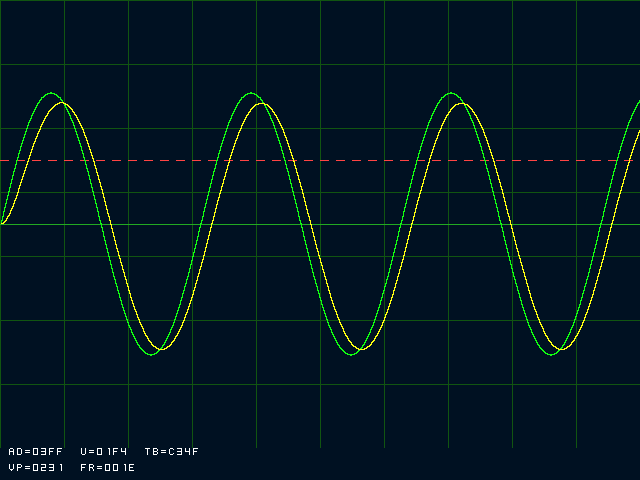
\includegraphics[width=0.78\linewidth]{../FPGA/src/vga/preview_640x480.png}
\caption{640$\times$480 显示效果（按 RTL 相同的映射关系复现）：双通道波形、64$\times$64 网格、
零电平轴、红色虚线为触发电平，底部两行为运行值。}
\label{fig:scope-preview}
\end{figure}

已知限制：（1）触发为“指针归零”式对齐，没有预触发深度与单次捕获；
（2）频率由帧内过零数 $\times$60 得到，分辨率 60Hz，且阈值固定为 512；
（3）滚动模式每帧更新一次基准，极高采样率下帧间会有跳变；
（4）串口命令为 ASCII 文本，极端情况下可能与二进制帧混淆；
（5）文本为固定模板，暂不支持任意字符串。

% =====================================================================
%  ch16_self_test.tex -- 第 16 章 屏幕自检程序解析
% =====================================================================
\section{屏幕自检程序解析（\file{vga_test_app.v} / \file{vga_test_top.v}）}

\subsection{设计目标与分层约束}

上板调试时，最怕“屏幕不亮却不知道是 FPGA、接线还是显示器的问题”。为此在
\textbf{应用层}增加一个与示波器功能完全解耦的自检程序：它不依赖 AD/DA 数据通路，
只使用系统时钟、复位与按键，把 5 幅标准测试画面送到 VGA 端口。

设计约束如下：

\begin{itemize}[leftmargin=2em,itemsep=2pt]
  \item 只新增两个上层文件，不修改 \file{hal/} 与 \file{abs/} 中任何封装；
  \item 复用已有接口：时序直接例化 \file{hal/vga_timing.v}，字模直接例化
        \file{hal/font_rom.v}，按键去抖直接例化 \file{app/scope_ui.v}；
  \item 输出级与 \file{vga_scope_top.v} 完全一致（2 拍 = 1 像素对齐），
        因此两种顶层可共用同一套引脚约束，切换 Top 不改 PCB。
\end{itemize}

\begin{table}[htbp]
\centering
\small
\caption{自检程序复用的下层模块}
\begin{tabular}{lllp{5.4cm}}
\toprule
模块 & 层 & 接口 & 用途\\
\midrule
\file{vga_timing.v} & HAL & \sig{clk/rst/pix_ce/hs/vs/de/px/py} & 产生 640$\times$480 时序与像素坐标\\
\file{font_rom.v} & HAL & \sig{ch/row/bits} & 8$\times$8 字模，用于第 5 幅文字画面\\
\file{scope_ui.v} & APP & \sig{key_in/ev_short} & 20ms 去抖 + 短按事件（切换画面）\\
\bottomrule
\end{tabular}
\end{table}

\subsection{\file{vga_test_top.v}：自检顶层}

\begin{center}
\small
\begin{tabular}{ll}
\toprule
项目 & 内容\\
\midrule
行数 & 132 行\\
端口 & \sig{clk/rst/key_in} 输入；\sig{vga_rgb[11:0]/vga_hs/vga_vs/vga_de} 输出\\
参数 & 与 \file{vga_scope_top.v} 相同的时序参数，外加 \sig{AUTO_FRAMES}（默认 120 帧）\\
\bottomrule
\end{tabular}
\end{center}

\subsubsection{块 1：时序例化（29--45 行）}

\begin{lstlisting}[style=vsnip]
vga_timing #(
    .H_VIS(H_VIS), .H_FP(H_FP), .H_SYNC(H_SYNC), .H_BP(H_BP),
    .V_VIS(V_VIS), .V_FP(V_FP), .V_SYNC(V_SYNC), .V_BP(V_BP),
    .H_POL(H_POL), .V_POL(V_POL), .PIX_DIV(PIX_DIV)
) u_timing (
    .clk(clk), .rst(rst), .pix_ce(pix_ce),
    .hs(hs), .vs(vs), .de(de), .px(px), .py(py)
);
\end{lstlisting}

自检顶层没有采样、没有缓存，直接把 HAL 时序的输出坐标交给图案发生器；参数全部
透传，所以换分辨率时与示波器一样只改顶层参数。

\subsubsection{块 2：帧起始脉冲（48--50 行）}

\begin{lstlisting}[style=vsnip]
reg vs_d;
always @(posedge clk) vs_d <= vs;
wire frame = vs & (~vs_d);
\end{lstlisting}

对场同步信号取上升沿，得到一个时钟宽的 \sig{frame} 脉冲。它驱动三件事：
自动换画面的计数、移动方块的推进、以及（示波器里的）滚动基准。本设计采用负极性
同步（\sig{V_POL=0}），场同步的上升沿正好落在消隐结束处，因此与“帧首”对齐。

\subsubsection{块 3：按键复用（52--64 行）}

\begin{lstlisting}[style=vsnip]
scope_ui #(.CLK_HZ(50_000_000), .DB_MS(20), .LONG_MS(800)) u_key (
    .clk(clk), .rst(rst), .key_in(key_in),
    .ev_short(ev_next), .ev_long(ev_long_unused)
);
\end{lstlisting}

直接复用示波器的按键模块，不重复实现消抖；长按事件在自检模式中不使用。

\subsubsection{块 4：图案例化（66--80 行）}

\begin{lstlisting}[style=vsnip]
vga_test_app #(
    .H_VIS(H_VIS), .V_VIS(V_VIS),
    .AUTO_FRAMES(AUTO_FRAMES), .COL_BG(COL_BG)
) u_app (
    .clk(clk), .rst(rst), .ev_next(ev_next), .frame(frame),
    .px(px), .py(py), .de(de), .rgb(rgb_comb), .mode_o()
);
\end{lstlisting}

图案模块只接收“当前像素坐标 + 有效区 + 事件”，返回该像素的颜色，属于典型的
\textbf{流式渲染}接口，不需要帧缓存。

\subsubsection{块 5：输出寄存与对齐（85--112 行）}

\begin{lstlisting}[style=vsnip]
always @(posedge clk) begin
    if (rst) begin rgb_r <= COL_BG; hs1 <= 1; hs2 <= 1; ... end
    else begin
        hs1 <= hs; hs2 <= hs1;
        vs1 <= vs; vs2 <= vs1;
        de1 <= de; de2 <= de1;
        if (pix_ce) rgb_r <= rgb_comb;
    end
end
\end{lstlisting}

像素在 \sig{pix_ce} 时打入寄存器，同步信号固定延迟 2 拍（因为像素周期为 2 个
时钟，正好等于 1 个像素），从而与 \sig{rgb_r} 对齐——与示波器顶层完全相同的处理，
保证两种顶层的时序行为一致。

\subsection{\file{vga_test_app.v}：图案发生器}

\begin{center}
\small
\begin{tabular}{ll}
\toprule
项目 & 内容\\
\midrule
行数 & 198 行\\
参数 & \sig{H_VIS=640}、\sig{V_VIS=480}、\sig{AUTO_FRAMES=120}、\sig{COL_BG}\\
端口 & \sig{clk/rst/ev_next/frame/px/py/de} 输入；\sig{rgb[11:0]}、\sig{mode_o[2:0]} 输出\\
\bottomrule
\end{tabular}
\end{center}

\subsubsection{块 1：模式与动画计数（40--76 行）}

\begin{lstlisting}[style=vsnip]
if (frame) begin
    pos <= (pos >= 10'd592) ? 10'd0 : (pos + 10'd4);
    if (auto_cnt == (AUTO_FRAMES-1)) begin
        auto_cnt <= 8'd0;
        mode     <= (mode == (NMODE-1)) ? 3'd0 : (mode + 3'd1);
    end
    else auto_cnt <= auto_cnt + 8'd1;
end
if (ev_next) begin
    mode     <= (mode == (NMODE-1)) ? 3'd0 : (mode + 3'd1);
    auto_cnt <= 8'd0;
end
\end{lstlisting}

\begin{itemize}[leftmargin=2em,itemsep=1pt]
  \item \sig{auto_cnt} 计满 \sig{AUTO_FRAMES}（默认 120 帧，约 2s）后切换画面；
  \item \sig{ev_next}（按键短按）立即切换并把自动计数清零，按键优先级更高；
  \item \sig{pos} 每帧加 4 像素，到 592（$640-48$，即方块刚好贴右边界）回卷到 0，
        因此移动方块在 2.5 秒左右扫过一屏。
\end{itemize}

\subsubsection{块 2：彩条画面（78--96 行）}

\begin{lstlisting}[style=vsnip]
wire [2:0] bar_idx = px[8:6];
always @(*) begin
    case (bar_idx)
        3'd0: bar_col = 12'hFFF;   // 白
        3'd1: bar_col = 12'hFF0;   // 黄
        ...
        default: bar_col = 12'h000; // 黑
    endcase
end
\end{lstlisting}

取像素列号的高 3 位（每 64 像素一段）作为色条索引，8 色轮转。由于 640 像素可分为
10 段，最后两段会重复白/黄，属于预期现象。该画面用于检查 \sig{vga_rgb[11:10]}、
\sig{[7:6]}、\sig{[3:2]} 与显示器 RGB 的对应关系以及电阻网络的电平。

\subsubsection{块 3：灰阶画面（98--101 行）}

\begin{lstlisting}[style=vsnip]
wire [3:0] gray_lvl = py[8:6];          // 0..7
wire [11:0] gray_col = {gray_lvl, gray_lvl, gray_lvl};
\end{lstlisting}

用行号的高 3 位产生 8 级灰度，R=G=B，用来判断三个通道的增益是否一致
（若某一级偏色，说明该通道的电阻比例或焊接有问题）。

\subsubsection{块 4：棋盘格（103--105 行）}

\begin{lstlisting}[style=vsnip]
wire chk = px[5] ^ py[5];
\end{lstlisting}

每 32 像素翻转一次，形成 32$\times$32 的黑白棋盘。该项对“像素时钟是否稳定、
行场同步是否抖动”最敏感：若出现斜纹、抖动或局部错位，通常是像素时钟或同步时序问题。

\subsubsection{块 5：边框、十字与移动方块（107--116 行）}

\begin{lstlisting}[style=vsnip]
wire border = (px < 4) || (px >= H_VIS-4) || (py < 4) || (py >= V_VIS-4);
wire cross  = ((py >= 238) && (py <= 241)) || ((px >= 318) && (px <= 321));
wire [11:0] box_x = {2'b00, pos};
wire moving = (px >= box_x) && (px < box_x + 48) && (py >= 200) && (py < 248);
\end{lstlisting}

4 像素宽的白色边框检查“满屏是否被裁切”，红色十字检查画面中心与几何比例，
48$\times$48 的绿色方块逐帧右移，用来确认帧刷新与无撕裂。

\subsubsection{块 6：文字画面（118--166 行）}

\begin{lstlisting}[style=vsnip]
wire in_t0 = (px >= tx0) && (px < tx0+64) && (py >= ty0) && (py < ty0+8);
wire in_t1 = (px >= tx1) && (px < tx1+96) && (py >= ty1) && (py < ty1+8);
...
wire [5:0] ch_sel  = in_t1 ? code1 : code0;
wire [2:0] row_sel = in_t1 ? r1 : r0;
font_rom u_font (.ch(ch_sel), .row(row_sel), .bits(font_bits));
wire [2:0] bit_idx = in_t1 ? (px - tx1) : (px - tx0);
wire text_hit = (in_t0 || in_t1) && font_bits[3'd7 - bit_idx];
\end{lstlisting}

两行文字“VGA TEST”与“640X480 60HZ”分别位于 $y=200$ 与 $y=232$，水平居中；
字符码由 \sig{case(col)} 常量表给出（V/G/A/空格/T/E/S 与 6/4/0/X/4/8/0/空格/6/0/H/Z），
只用一个 \file{font_rom} 实例，按“当前所在行”多路选择输入，因此字模资源只有一份。

\subsubsection{块 7：画面选择（168--186 行）}

\begin{lstlisting}[style=vsnip]
always @(*) begin
    if (!de) rgb = COL_BG;
    else case (mode)
        3'd0: rgb = bar_col;
        3'd1: rgb = gray_col;
        3'd2: rgb = chk ? 12'hFFF : 12'h000;
        3'd3: rgb = border ? 12'hFFF : cross ? 12'hF00 : moving ? 12'h0F0 : COL_BG;
        3'd4: rgb = text_hit ? 12'hFFF : COL_BG;
        default: rgb = COL_BG;
    endcase
end
\end{lstlisting}

消隐区（\sig{de=0}）统一输出背景色，避免把随机颜色带到消隐期；五个画面通过
\sig{mode} 选择，全部为组合逻辑。

\subsection{自检画面的判读方法}

\begin{table}[htbp]
\centering
\small
\caption{自检画面与对应的硬件检查点}
\begin{tabular}{clp{7.8cm}}
\toprule
编号 & 画面 & 检查点\\
\midrule
0 & 8 色竖条 & RGB 三路是否都在、位序是否正确、颜色是否饱和\\
1 & 8 级灰阶 & 灰阶是否单调、有无台阶丢失（位宽/电阻比例）\\
2 & 棋盘格 & 像素时钟与行场同步是否稳定、有无撕裂/斜纹\\
3 & 边框+十字+方块 & 满屏是否被 overscan 裁切、中心是否居中、动画是否流畅\\
4 & 文字 & 字模取字是否正确、像素是否 1:1 对齐\\
\bottomrule
\end{tabular}
\end{table}

\begin{table}[htbp]
\centering
\small
\caption{常见现象与原因对照}
\begin{tabular}{p{4.2cm}p{9.6cm}}
\toprule
现象 & 可能原因\\
\midrule
全黑、显示器提示无信号 & HS/VS（T11/T12）未接、接反或极性错；先量同步脚\\
有画面但偏色/缺色 & RGB 某一位未接、270$\Omega$/560$\Omega$ 接反、BankVccio 不是 3.3V\\
画面滚动、斜纹 & 像素时钟不对（确认 50MHz 与 \sig{PIX_DIV=2}）或同步极性错\\
只有部分区域或偏移 & 显示器 overscan，或时序参数与该显示器支持的模式不符\\
棋盘闪烁/抖动 & 电源纹波、时钟质量、VGA 线材过长\\
\bottomrule
\end{tabular}
\end{table}

\subsection{资源与验证}

图案发生器除模式计数与移动计数器外均为组合逻辑，估计约 400 LUT（不含时序模块），
占用 2 个 8bit 字模行查询和一个 12bit 输出寄存器，不占 BSRAM 与 DSP。

验证结果：

\begin{itemize}[leftmargin=2em,itemsep=1pt]
  \item TD 6.0.3 前端分析：27 个源文件全部通过（含本章两个文件），
        仅剩原工程既有的 \sig{BAUD_CNT_MAX} 提示；
  \item 自写端口连接检查：25 个模块、31 处例化，0 个未定义端口；
  \item 未做 RTL 仿真与上板：上板时建议先烧 \sig{TEST_MODE=1} 版本确认屏幕，
        再切回示波器功能。
\end{itemize}

\subsection{完整注释源码}

\lstinputlisting[style=vcode]{../FPGA/src/vga/vga_test_top.v}

\lstinputlisting[style=vcode]{../FPGA/src/vga/app/vga_test_app.v}

% =====================================================================
%  ch17_fixes.tex -- 第 17 章 缺陷修复分支（fix/review-p1-p11）
% =====================================================================
\section{缺陷修复分支（fix/review-p1-p11）}

\subsection{分支约定与回退方法}

第 2--13 章描述的是 \textbf{main 分支}上的原始设计；本章描述从 main 切出的修复分支
\textbf{fix/review-p1-p11} 中的改动。为保证正文（尤其完整源码清单）与所描述的版本一致，
第 2、4、5、9、10、13 章的源码清单已改为引用
\file{doc/baseline/} 下从 main 导出的副本，本章则展示修复后的代码片段。

\begin{center}
\small
\begin{tabular}{ll}
\toprule
项目 & 内容\\
\midrule
仓库 & \url{https://github.com/starfruitsz/FPGA}\\
分支 & \file{fix/review-p1-p11}（基于 main 的 \sig{00a614c}）\\
提交 & \sig{27694bf}（整批修复）、\sig{a63401d}（P9 回撤）、\sig{b34fff3}（P5 模式开关）\\
回退 & \sig{git checkout main}；或对单个提交 \sig{git revert <commit>}\\
基线源码 & \file{doc/baseline/}（main 上的 adda/eso/divider/seg/bcd/cst 副本）\\
\bottomrule
\end{tabular}
\end{center}

\subsection{修复清单}

\begin{table}[htbp]
\centering
\small
\caption{缺陷与修复一览}
\begin{tabular}{clp{7.4cm}}
\toprule
编号 & 文件 & 修复内容\\
\midrule
P1 & \file{eso.v} & 参数锁存由 \sig{if/else-if} 优先级改为两个独立 \sig{if}，k 参数不再被“锁死”\\
P2 & \file{eso.v} & 符号项 \sig{4'b1111}（补零后为 +15）改为 \sig{5'sd1 / -5'sd1}，恢复真正的 $\pm1$\\
P3 & — & 复核后\textbf{撤销}：32bit 与 22bit 有符号相加只需 33bit，\sig{she} 宽度足够\\
P4 & \file{bcd.v}、\file{seg.v} & BCD 扩展到 4 位并新增 \sig{thou}；seg 增加“千位优先”显示分支\\
P5 & \file{adda.v}、\file{adda_scope_top.v} & 新增 \sig{UART_MODE} 开关（连续/标志位）与可配置 \sig{REPORT_MS} 上报周期\\
P6 & \file{seg.v} & \sig{sel <= ~sel_reg[3:0]}，去掉隐式截断\\
P7 & \file{seg.v} & 小数点索引加越界保护，仿真不再读 X\\
P8 & \file{divider.v} & “500 分频”注释更正为 50000 分频\\
P9 & — & \textbf{已回撤}：按需求保留 \sig{ad_clk}/\sig{da_clk} 输入端口（未使用，综合会裁剪）\\
P10 & \file{adda.v} & 删除 \sig{initial}，改在块 5 的复位分支清 \sig{po_flag2}\\
P11 & \file{.cst} & 补数码管 \sig{sel}/\sig{seg} 共 12 个引脚约束\\
P12 & \file{.gprj} & 从工程文件列表移除未例化的 \file{gowin_pll.v}/\file{fifo_top.v}\\
\bottomrule
\end{tabular}
\end{table}

\subsection{逐项代码解析}

\subsubsection{P1：参数更新优先级}

修复前（main）：

\begin{lstlisting}[style=vsnip]
else if(c_flag==1'b1)
    c<=c_date;
else if(k_flag==1'b1)
    k<=k_date;
else
    begin c<=c; k<=k; end
\end{lstlisting}

顶层把两个标志置 1 后都不清零（这是有意为之——它要跨到 1kHz 的 \sig{ad_clk} 域，
脉冲会丢），于是 \sig{c_flag} 一旦为 1，\sig{else if} 分支永远进不去，k 参数再也改不了。
修复后改为两个互不排斥的独立 \sig{if}：

\begin{lstlisting}[style=vsnip]
if(c_flag==1'b1)
    c<=c_date;
if(k_flag==1'b1)
    k<=k_date;
\end{lstlisting}

两个标志同时有效时 c、k 都更新；都无效时寄存器自动保持（\sig{always} 块特性），
既保留了电平式跨时钟域的做法，又消除了优先级导致的功能失效。

\subsubsection{P2：符号项 sgn}

\begin{lstlisting}[style=vsnip]
// 修复前
wire signed [4 : 0] sgn;
assign sgn = (she>1'd0) ? 1'd1 : 4'b1111;   // 4'b1111 补零后 = +15

// 修复后
assign sgn = (she > 0) ? 5'sd1 : -5'sd1;     // 真正的 +1 / -1
\end{lstlisting}

该改动会改变闭环控制律的偏置项，属于行为变化，切换后需要重新整定 \sig{c}/\sig{k}。

\subsubsection{P4：4 位 BCD 与显示}

原实现只保留 3 位 BCD（0$\sim$999），AD 码值 1000$\sim$1023 会丢掉千位。
修复后移位寄存器由 22bit 扩到 26bit（16bit BCD + 10bit 二进制），加 3 修正从 3 组变 4 组：

\begin{lstlisting}[style=vsnip]
reg [25:0] data_shift;
...
data_shift[13:10] <= (data_shift[13:10] > 4) ? data_shift[13:10] + 2'd3 : data_shift[13:10];
data_shift[17:14] <= ...;   data_shift[21:18] <= ...;
data_shift[25:22] <= (data_shift[25:22] > 4) ? data_shift[25:22] + 2'd3 : data_shift[25:22];
...
thou <= data_shift[25:22];
\end{lstlisting}

用同样的算法做软件复算，$0/9/99/999/1000/1023$ 均正确（例如 1023 $\rightarrow$ 1\,0\,2\,3）。
\file{seg.v} 中新增最高优先级的显示分支：

\begin{lstlisting}[style=vsnip]
else if(thou != 4'd0)
    data_reg <= {thou,hun,ten,unit};     // 4 位数字，最左位是千位（不显示负号）
\end{lstlisting}

\subsubsection{P5：串口上报方式与速率}

\file{adda.v} 新增三个参数，\sig{CNT_MAX} 由周期自动推导：

\begin{lstlisting}[style=vsnip]
parameter integer UART_MODE = 1,          // 0=连续发送 1=按标志位
parameter integer CLK_FREQ  = 50_000_000,
parameter integer REPORT_MS = 26,         // 上报周期(ms)
parameter integer CNT_MAX   = (CLK_FREQ/1000)*REPORT_MS - 1;

wire tx_req = (UART_MODE != 0) ? pi_flag : 1'b1;   // 模式选择
...
    .pi_flag(tx_req)                                // 送 uart_tx
\end{lstlisting}

计数器由 25bit 加宽到 32bit，支持最长约 85 秒的周期；\sig{UART_MODE} 为常数，
未被选中的分支会被综合常量折叠。\file{adda_scope_top.v} 把两个参数透传到顶层：

\begin{center}
\small
\begin{tabular}{lll}
\toprule
模式 & 参数 & 效果\\
\midrule
连续发送（旧行为） & \sig{UART_MODE=0} & 发送器不停机，占满串口带宽\\
定时上报（默认） & \sig{UART_MODE=1, REPORT_MS=26} & 每 26ms 一帧，约 38 帧/s\\
高速上报 & \sig{UART_MODE=1, REPORT_MS=5} & 每 5ms 一帧\\
低速上报 & \sig{UART_MODE=1, REPORT_MS=200} & 每 200ms 一帧\\
\bottomrule
\end{tabular}
\end{center}

50MHz 下的计数值：26ms $\rightarrow$ 1\,299\,999；10ms $\rightarrow$ 499\,999；
100ms $\rightarrow$ 4\,999\,999。

\subsubsection{P6/P7：数码管细节}

\begin{lstlisting}[style=vsnip]
// P6：显式取低 4 位，不再依赖隐式截断
sel <= ~sel_reg[3:0];

// P7：point 只有 4bit，cnt_sel 可到 5，越界索引会读到 X
dot_disp <= (cnt_sel <= 3'd3) ? point[cnt_sel[1:0]] : 1'b0;
\end{lstlisting}

\subsubsection{P9 回撤与 P10/P8/P12}

\begin{itemize}[leftmargin=2em,itemsep=2pt]
  \item \textbf{P9 已回撤}：按需求保留 \sig{ad_clk}/\sig{da_clk} 输入端口（顶层与 \sig{adda}
        均恢复），端口未使用、综合时会自动裁剪，不增加资源；
  \item \textbf{P10}：删除 \sig{initial} 初值，改为在块 5 复位分支中写
        \sig{po_flag2<=1'b0}，不再依赖器件上电初值特性；
  \item \textbf{P8}：\file{divider.v} 参数行注释由“500 分频”更正为“50000 分频（50MHz$\rightarrow$1kHz）”；
  \item \textbf{P12}：\file{.gprj} 的 FileList 移除未例化的 PLL/FIFO（文件仍保留在仓库）。
\end{itemize}

\subsubsection{P11：数码管引脚约束}

原工程只约束了 30 个引脚，\sig{sel[3:0]}/\sig{seg[7:0]} 是 PnR 自动布局的。
修复后把实测引脚写入 \file{.cst}，约束总数变为 50 个：

\begin{table}[htbp]
\centering
\small
\begin{tabular}{lcccccccc}
\toprule
信号 & seg[0] & seg[1] & seg[2] & seg[3] & seg[4] & seg[5] & seg[6] & seg[7]\\
\midrule
引脚 & U18 & L14 & P16 & V16 & P12 & N15 & V13 & R11\\
\midrule
信号 & sel[0] & sel[1] & sel[2] & sel[3] & \multicolumn{4}{c}{}\\
\midrule
引脚 & N16 & U17 & N14 & T17 & \multicolumn{4}{c}{}\\
\bottomrule
\end{tabular}
\end{table}

\subsection{验证与上板注意事项}

\begin{center}
\small
\begin{tabular}{ll}
\toprule
检查 & 结果\\
\midrule
TD 6.0.3 前端分析 & 27 个源文件通过\\
端口连接静态检查 & 25 个模块、31 处例化、0 个未定义端口\\
约束文件 & 50 个端口 / 50 个唯一引脚，无重复\\
4 位 BCD 算法 & Python 复算 0/9/99/999/1000/1023 全部正确\\
逻辑综合/时序/上板 & 待 Gowin EDA 与实板完成\\
\bottomrule
\end{tabular}
\end{center}

\begin{warnbox}
\textbf{行为变化提醒}：（1）P2 改变了控制律的偏置项，闭环动态会变，需重新整定
$c$、$k$；（2）P5 默认从“连续发送”改为“26ms 一帧”，上位机若按连续流设计需要调整；
（3）P4 在 $\ge$1000 时显示 4 位数字且不显示负号；（4）P9 回撤后端口数量与 main 一致。
\end{warnbox}

% =====================================================================
%  ch18_scope_v2.tex -- 第 18 章 示波器应用层增强（v2）
% =====================================================================
\section{示波器应用层增强（v2）}

本章记录 \file{fix/review-p1-p11} 分支上的第二次功能升级：在不改动 HAL/ABS 封装的前提下，
把采集层升级为带触发状态机的结构，并扩展测量与文本显示。对应提交见仓库
\url{https://github.com/starfruitsz/FPGA} 的 \file{fix/review-p1-p11} 分支。

\section{设计目标}

\begin{enumerate}[leftmargin=2em,itemsep=2pt]
  \item 触发从“单一边沿 + 指针归零”升级为 \textbf{状态机 + 模式 + 预触发 + 保持时间}；
  \item 测量从“Vpp/频率”扩展到 \textbf{最大/最小/均值/周期/占空比}；
  \item 文本层从固定 5 字段升级为 \textbf{双页轮显}；
  \item 增加 \textbf{PC 上位机 MVP} 与 \textbf{MIT 许可}；
  \item 所有改动只落在 APP 层与顶层，HAL/ABS 接口保持不变（除文本层新增 \sig{page} 端口）。
\end{enumerate}

\section{触发状态机}

采集层（\file{scope_capture.v}）内部改为 4 状态机：

\begin{center}
\small
\begin{tabular}{cll}
\toprule
状态 & 名称 & 行为\\
\midrule
\sig{2'd0} & IDLE & 等待 \sig{arm}，不写 RAM\\
\sig{2'd1} & ARMED & 自由写入循环缓冲，等待触发条件\\
\sig{2'd2} & FILL & 已触发，继续写满一屏（\sig{1<<DEPTH_LOG2} 个点）\\
\sig{2'd3} & DONE & 停止写入，等待下一次 \sig{arm}\\
\bottomrule
\end{tabular}
\end{center}

\subsection{触发模式}

\begin{center}
\small
\begin{tabular}{clp{6.6cm}}
\toprule
\sig{trig_mode} & 名称 & 行为\\
\midrule
\sig{2'd0} & auto & 自由滚动显示；触发只更新对齐基准 \sig{rd_base}，不停机\\
\sig{2'd1} & normal & 触发后填满一屏进入 DONE；APP 检测到 \sig{done} 自动重新 \sig{arm}，连续刷新\\
\sig{2'd2} & single & 触发一次后停在 DONE，必须按键或串口 \sig{arm} 才继续\\
\bottomrule
\end{tabular}
\end{center}

\subsection{预触发与保持时间}

触发命中时锁存显示基准：

\begin{lstlisting}[style=vsnip]
rd_base <= waddr - pre_trig;   // 显示起点前移，屏幕上可见触发点之前的波形
hold_cnt <= holdoff;           // 之后 holdoff 个采样点内忽略新触发
\end{lstlisting}

显示读地址 = \sig{rd_base + px}。由于缓冲区是循环写入的，\sig{rd_base} 之前的地址里
正好是触发前的历史采样，因此不需要额外的“预触发存储”。

\section{扩展测量}

\file{scope_meas.v} 在每帧内并行统计：

\begin{center}
\small
\begin{tabular}{llp{6.2cm}}
\toprule
输出 & 位宽 & 计算方式\\
\midrule
\sig{vpp} & 10 & 帧内 \sig{vmax} $-$ \sig{vmin}\\
\sig{vmax}/\sig{vmin} & 10 & 采样比较器\\
\sig{vmean} & 10 & 前 256 点累加和右移 8 位（避免除法器）\\
\sig{period} & 16 & 相邻上升穿越之间的采样点数\\
\sig{freq} & 16 & 帧内上升穿越次数 $\times 60$（帧频约 60Hz）\\
\sig{duty} & 8 & 前 256 点中高于阈值的比例（0$\sim$100）\\
\bottomrule
\end{tabular}
\end{center}

RMS 需要开方，本版未实现；后续可用 CORDIC 或查表。

\section{双页文本}

文本层新增 \sig{page} 输入，模板变为两页（列位置两页一致）：

\begin{center}
\small
\begin{tabular}{cll}
\toprule
页 & 第 0 行 & 第 1 行\\
\midrule
0 & \sig{AD=####  U=####  TB=####} & \sig{VP=####  FR=####}\\
1 & \sig{HI=#### LO=####  AV=####} & \sig{PE=#### DU=####}\\
\bottomrule
\end{tabular}
\end{center}

\sig{page} 由 APP 每 2 秒翻转一次，顶层按页把不同的值接到 \sig{val0..val4}。

\section{串口协议}

新增 4 条命令（原有 T/R/A/L/E/S 不变），格式仍为 \sig{<字母><十六进制><CR/LF>}：

\begin{center}
\small
\begin{tabular}{lll}
\toprule
命令 & 含义 & 取值范围\\
\midrule
\sig{M<hex>} & 触发模式 & 0=auto 1=normal 2=single\\
\sig{C<hex>} & 触发源 & 0=CH0 1=CH1\\
\sig{P<hex>} & 预触发点数 & 0$\sim$3FF\\
\sig{H<hex>} & 保持时间 & 0$\sim$FFFF 采样点\\
\bottomrule
\end{tabular}
\end{center}

\section{上位机 MVP}

\file{tools/scope_host.py}：

\begin{lstlisting}[style=vsnip]
python scope_host.py --port COM3 --baud 115200        # 实时波形
python scope_host.py --port COM3 --csv cap.csv        # 存 CSV
\end{lstlisting}

按“先低字节、后高字节”还原 10bit 码值（\sig{lo | ((hi & 3) << 8)}），用 matplotlib 滚动显示。

\section{验证与限制}

\begin{center}
\small
\begin{tabular}{ll}
\toprule
项 & 结果\\
\midrule
TD 前端分析 & 27 个文件通过\\
端口连接检查 & 25 模块 / 31 例化 / 0 错误\\
仿真 & 未做\\
上板 & 未做（需实测状态机与预触发偏移）\\
ETS 等效采样 & 未实现（需 PLL 相位或延时链）\\
\bottomrule
\end{tabular}
\end{center}

\begin{warnbox}
本版改动集中在 \file{scope_capture.v}、\file{scope_meas.v}、\file{scope_app.v}、
\file{scope_cmd.v}、\file{text_layer.v} 与 \file{vga_scope_top.v}；
上板前建议先把 \sig{FEAT_TRIG} 置 0 验证显示通路，再打开触发逐项试验。
\end{warnbox}

% =====================================================================
%  ch19_sparkroad.tex -- 第 19 章 SparkRoad-V 移植与 TD 工程操作
% =====================================================================
\section{SparkRoad-V 移植与 TD 工程操作}

本章记录把示波器从高云 GW5A 工程迁移到 \textbf{SparkRoad-V（Anlogic EG4S20BG256）}
的顶层设计、引脚约束生成方式，以及完整的 TD 工程操作步骤。

\subsection{目标板与器件}

\begin{center}
\small
\begin{tabular}{ll}
\toprule
项目 & 参数\\
\midrule
FPGA & Anlogic EG4S20BG256（Eagle 系列，BG256）\\
系统时钟 & 24\,MHz 有源晶振（K14）\\
VGA & GM7123 视频 DAC，24\,bit（RGB 各 8\,bit），HS/VS/CLK\\
ADC & AD7606 模块（8 通道 16\,bit、200\,kSPS、±5V/±10V、SPI/并口）\\
数码管 & 4 位，DIG\_1..4 + SEG\_A..H\\
按键 & 5 个独立按键（BUTTON\_L/R/U/D/C）\\
串口 & USB2UART（TX=F16，RX=E16）\\
\bottomrule
\end{tabular}
\end{center}

\subsection{顶层结构}

\file{sparkroad_scope_top.v} 的组成：

\begin{center}
\small
\begin{tabular}{lll}
\toprule
模块 & 作用 & 说明\\
\midrule
\file{uart_rx} & 接收 115200 字节 & 24\,MHz 时钟\\
\file{scope_cmd} & 示波器命令（T/R/A/L/E/S/M/C/P/H） & 产生 cfg 写脉冲\\
\file{adc_cmd} & ADC 命令（R/O/S/K/N） & 产生 CSR 写\\
\file{adc_ad7606_top} & AD7606 串行采集 + 归一化 & 10\,bit 输出\\
\file{vga_scope_top} & 示波器显示 & 640$\times$480，PIX\_DIV=1\\
\file{seg} & 数码管显示 AD 码值 & 4 位动态扫描\\
\file{uart_tx} & 每 1\,ms 上报一帧 & 16\,bit\\
\bottomrule
\end{tabular}
\end{center}

信号流：AD7606 $\rightarrow$ ADC HAL（补码$\rightarrow$偏移二进制$\rightarrow$10\,bit）
$\rightarrow$ 采集/触发/测量 $\rightarrow$ 图层合成 $\rightarrow$ VGA RGB444
$\rightarrow$ 每 4\,bit 复制为 8\,bit $\rightarrow$ GM7123。

\subsection{时钟与视频时序}

\begin{itemize}[leftmargin=2em,itemsep=2pt]
  \item 板载时钟 24\,MHz，直接作为像素时钟（\sig{PIX_DIV=1}）；
  \item 640$\times$480 行场参数：H=640+16+96+48=800，V=480+10+2+33=525；
  \item 场频 = 24\,MHz / (800$\times$525) $\approx$ 57.1\,Hz，属于显示器可接受范围；
  \item 若要严格 59.94\,Hz，可用 PLL 产生 25.175\,MHz（需要 EG4 的 PLL IP）。
\end{itemize}

\subsection{引脚与约束生成}

引脚不再手写约束，而是集中在一个 CSV：

\begin{lstlisting}[style=vsnip]
FPGA/src/adc/pins/board_pins.csv   # 信号,位宽,引脚(|分隔),说明
tools/gen_adc_pins.py              # -> FPGA_TD/eg4/SparkRoad.adc
\end{lstlisting}

CSV 覆盖 20 个信号、51 个引脚（时钟、复位、按键、串口、VGA 24\,bit、
数码管、AD7606 七根线）。修改接线只改 CSV，再运行脚本重新生成；
脚本会检查位宽匹配与引脚重复。

\subsection{TD 工程操作步骤}

\subsubsection{环境要求}

TD 必须安装 \textbf{Eagle（EG4）器件库}。若打开工程提示
\sig{Unknown device name EG4S20BG256}，说明当前 TD 只有 PH1/PH2 器件库
（本机 TD 6.0.3 即如此），需安装 TD 5.x 或向 Anlogic 索取 EG4 支持包。

\subsubsection{创建工程（Tcl）}

\begin{lstlisting}[style=vsnip]
cd <repo>/FPGA_TD/eg4
create_project -family eg4 -device EG4S20BG256 EG4S20BG256_scope .
import_device eg4_20.db -package BG256 -speed 5
add_files -list ./files.list
top_module sparkroad_scope_top
exit
\end{lstlisting}

\subsubsection{图形界面步骤}

\begin{enumerate}[leftmargin=2em,itemsep=2pt]
  \item 打开 \file{FPGA_TD/EG4S20BG256_scope.al}（或按上节重建）；
  \item 确认器件为 \sig{EG4S20BG256}，速度等级与板卡一致（默认 -5）；
  \item 源文件应为 \textbf{37 个}，顶层设为 \sig{sparkroad_scope_top}；
  \item 在约束集里加入 \file{FPGA_TD/eg4/SparkRoad.adc}；
  \item Run Synthesis $\rightarrow$ Run Place \& Route $\rightarrow$ Generate Bitstream；
  \item 用 TD Programmer 下载 \file{.bit} 到板卡。
\end{enumerate}

\subsubsection{约束文件格式}

Anlogic TD 使用 \file{.adc}，每行一条：

\begin{lstlisting}[style=vsnip]
set_pin_assignment {clk} { LOCATION = K14; IOSTANDARD = LVCMOS33; }
set_pin_assignment {vga_r[0]} { LOCATION = L5; IOSTANDARD = LVCMOS33; }
\end{lstlisting}

\subsection{上板调试顺序}

\begin{enumerate}[leftmargin=2em,itemsep=2pt]
  \item 先断开 AD7606，烧录工程，确认 VGA 出现网格/文字（证明时钟、VGA、
        图层链路正常）；
  \item 接 AD7606 的 5V/GND 与七根信号线，串口发 \sig{N1} 使能、\sig{R1} 选 ±10V；
  \item 给 IN1 输入 1\,kHz 正弦，观察波形；用 \sig{K} 调整采样间隔；
  \item 再测试触发（\sig{A1}、\sig{L}、\sig{M}）与预触发（\sig{P}）。
\end{enumerate}

\subsection{串口命令}

\begin{center}
\small
\begin{tabular}{lll}
\toprule
命令 & 作用 & 范围\\
\midrule
\sig{T<hex>} & 时基分频 & 0$\sim$FFFF\\
\sig{R<hex>} & 运行/冻结（scope） & 0/1\\
\sig{A<hex>} & 触发使能 & 0/1\\
\sig{L<hex>} & 触发电平 & 0$\sim$3FF\\
\sig{E<hex>} & 触发边沿 & 0/1\\
\sig{S<hex>} & 滚动开关 & 0/1\\
\sig{M<hex>} & 触发模式 & 0/1/2\\
\sig{C<hex>} & 触发源 & 0/1\\
\sig{P<hex>} & 预触发点数 & 0$\sim$3FF\\
\sig{H<hex>} & 保持时间 & 0$\sim$FFFF\\
\midrule
\sig{R<hex>} & ADC 量程（adc\_cmd） & 0=±5V 1=±10V\\
\sig{O<hex>} & 过采样 & 0$\sim$6\\
\sig{S<hex>} & SCLK 半周期 & 0$\sim$FFFF\\
\sig{K<hex>} & ADC 采样间隔 & 0$\sim$FFFF\\
\sig{N<hex>} & ADC 使能 & 0/1\\
\bottomrule
\end{tabular}
\end{center}

注意：\sig{R/S} 在示波器与 ADC 两个解析器中含义不同，但作用对象不同
（一个写 VGA 参数，一个写 ADC CSR），互不影响。

\subsection{已知限制}

\begin{itemize}[leftmargin=2em,itemsep=2pt]
  \item SparkRoad-V 无 DAC，CH1 暂接固定中点，仅 CH0 有效；
  \item AD7606 串行模式当前只读 DOUTA 的 ch1$\sim$ch4（ch5$\sim$8 需接 DOUTB）；
  \item 24\,MHz 像素时钟下场频约 57\,Hz，部分显示器可能需要 25.175\,MHz PLL；
  \item 本机 TD 6.0.3 缺 EG4 器件库，尚未实际综合/上板。
\end{itemize}

\subsection{验证}

\begin{center}
\small
\begin{tabular}{ll}
\toprule
项 & 结果\\
\midrule
TD 前端分析 & 37 个源文件通过\\
端口连接检查 & 35 模块 / 47 处例化 / 0 错误\\
约束生成 & 20 信号 / 51 引脚，无重复\\
综合/上板 & 待具备 EG4 器件库的 TD 环境\\
\bottomrule
\end{tabular}
\end{center}

% =====================================================================
%  appendix.tex
% =====================================================================
\appendix
\section{附录}

\subsection{附录 A：文件清单与统计}

\begin{table}[htbp]
\centering
\small
\begin{tabular}{llrr}
\toprule
文件 & 模块 & 原始行数 & 注释后行数\\
\midrule
\file{src/adda.v} & \texttt{adda} & 261 & 417\\
\file{src/rtl.v} & \texttt{rtl} & 80 & 143\\
\file{src/eso.v} & \texttt{eso} & 140 & 252\\
\file{src/divider.v} & \texttt{divider} & 50 & 82\\
\file{src/key.v} & \texttt{key} & 32 & 61\\
\file{src/seg.v} & \texttt{seg} & 153 & 231\\
\file{src/bcd.v} & \texttt{bcd} & 62 & 98\\
\file{src/uart_rx.v} & \texttt{uart\_rx} & 116 & 187\\
\file{src/uart_tx.v} & \texttt{uart\_tx} & 84 & 136\\
\file{src/gowin_pll/gowin_pll.v} & \texttt{Gowin\_PLL} & 137 & 171\\
\file{src/fifo_top/fifo_top.v} & \texttt{fifo\_top} & 504 & 536\\
\file{src/project_2025_11_07.cst} & 约束 & 69 & 109\\
\file{src/gowin_pll/gowin_pll_tmp.v} & 模板 & 19 & 30\\
\file{src/fifo_top/fifo_top_tmp.v} & 模板 & 24 & 34\\
\bottomrule
\end{tabular}
\end{table}

全部注释只增加以 \sig{//} 开头的整行注释，未改动任何代码行。经脚本比对，
注释前后去掉注释后的 Verilog 词法内容\textbf{完全一致}（17 个文件全部通过）。

\subsection{附录 B：模块与关键信号速查}

\begin{table}[htbp]
\centering
\small
\begin{tabular}{lll}
\toprule
模块 & 输入 & 输出\\
\midrule
\texttt{adda} & \sig{ad_date, key_in, rx, sys_clk, sys_rst_n} & \sig{ad_out, sel, seg, tx, led*, \*_clk1}\\
\texttt{rtl} & \sig{ad_data} & \sig{sign, volt}\\
\texttt{eso} & \sig{e_in, u_out, c/k} & \sig{out_da, z1k0..z3k0}\\
\texttt{divider} & \sig{sys_clk} & \sig{clk0, clk1}\\
\texttt{key} & \sig{key_in} & \sig{key_out}\\
\texttt{seg} & \sig{data, point, sign} & \sig{sel, seg}\\
\texttt{bcd} & \sig{data[9:0]} & \sig{unit, ten, hun}\\
\texttt{uart\_rx} & \sig{rx} & \sig{po_data, po_flag}\\
\texttt{uart\_tx} & \sig{pi_data, pi_flag} & \sig{tx}\\
\bottomrule
\end{tabular}
\end{table}

\subsection{附录 C：复现步骤}

\subsubsection{C.1 用安路 TD 打开（代码浏览用容器工程）}

高云 \sig{.gprj} 无法被 TD 直接打开，本报告用 TD 的 Tcl 接口创建了一个同名容器工程：

\begin{lstlisting}[style=cfgcode,numbers=none]
$env:PATH  # 需能找到 D:\FPGA\bin\td_commands_prompt.exe
cd C:/Users/Administrator/Desktop/task/FPGA_TD
# 通过 stdin 喂给 TD 的 Tcl 解释器：
create_project -family ph1 -device PH1A60GEG324 project_2025_11_07_TD .
import_device ph1_60.db -package PH1A60GEG324
add_files -list ./files.list
exit
\end{lstlisting}

随后直接双击 \file{project_2025_11_07_TD.al} 或
\sig{td.exe project_2025_11_07_TD.al} 即可打开，工程只引用 \file{../FPGA/src} 下的源文件，
不复制。注意该工程只能浏览/编辑代码，\textbf{不能}用安路器件综合本设计。

\subsubsection{C.2 编译本报告}

\begin{lstlisting}[style=cfgcode,numbers=none]
cd C:/Users/Administrator/Desktop/task/doc
xelatex main.tex
xelatex main.tex      # 第二遍生成目录与交叉引用
\end{lstlisting}

需要 MiKTeX（含 ctex 宏包与中文字体）。文档引用 \file{../FPGA/src/*.v} 源文件，
移动目录结构后需同步修改相对路径。

\subsection{附录 D：术语表}

\begin{table}[htbp]
\centering
\small
\begin{tabular}{ll}
\toprule
术语 & 含义\\
\midrule
ADRC & 自抗扰控制（Active Disturbance Rejection Control）\\
ESO & 扩张状态观测器（Extended State Observer），估计状态与总扰动\\
TD & 安路科技开发工具 TangDynasty\\
GW5A & 高云 Arora V 系列 FPGA（22nm 工艺）\\
8N1 & UART 8 数据位、无校验、1 停止位\\
FWFT & First-Word Fall-Through，FIFO 首字直通模式\\
BCD & 二进制编码十进制\\
LSB/MSB & 最低有效位 / 最高有效位\\
\bottomrule
\end{tabular}
\end{table}


\end{document}
